\section{线性空间和线性变换}

\subsection{线性空间}

\begin{definition}[映射,变换,函数]
设有集合 $S,S'$,定义规则 $\sigma:S\to S'$,使得集合 $S$ 中元素 $a$ 与 $S'$ 中唯一元素对应,记作:
\[
a'=\sigma(a)\quad\text{或}\quad \sigma:a\mapsto a'
\]
则称 $\sigma$ 为一个映射。特别地,若 $S$ 与 $S'$ 相同,则称 $\sigma$ 为变换;若 $S'$ 为数域,则称 $\sigma$ 为函数。
\end{definition}
\begin{com}
映射最本质的特征在于对于 $S$ 中的任意一个元素在 $S'$ 中仅有唯一的一个元素和它对应。
\end{com}

\begin{definition}[集值映射]
由单点映射 $\sigma:S\to S'$ 可导出集值映射 $\sigma:2^S\to 2^{S'}$,
\begin{align*}
    \sigma(\Omega)&=\{y:y=\sigma(x),\exists\,x\in\Omega\},\quad\forall\,\Omega\subset S\\
    \sigma^{-1}(\Omega')&=\{x:y=\sigma(x),\exists\,y\in\Omega'\},\quad\forall\,\Omega'\subset S'
\end{align*}
如图所示:
\begin{figure}[H]
    \centering
    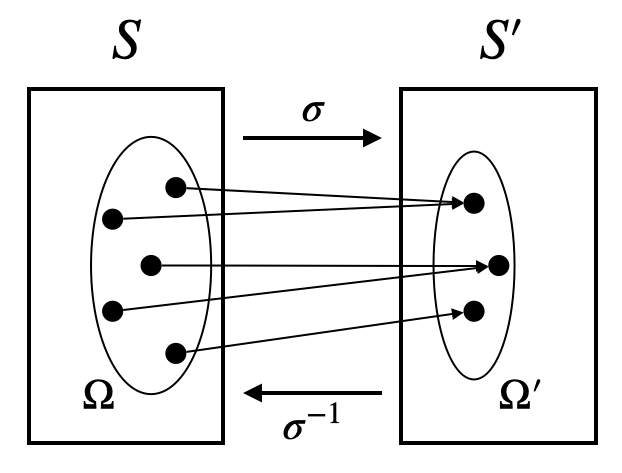
\includegraphics[width=0.25\linewidth]{figs/set-proj.png}
\end{figure}

\end{definition}

\begin{property}[集值映射的基本性质]
集值映射满足如下基本性质:
\begin{itemize}
    \item 任给子集 $\Omega\subset S$,则 $\sigma^{-1}(\sigma(\Omega))=\Omega$.
    \item 任给子集 $\Omega'\subset S'$,则 $\sigma(\sigma^{-1}(\Omega'))=\Omega'\cap \sigma(S)$.
\end{itemize}
如果用包含关系定义子集间的偏序关系,那么由映射导出的集值映射是保持这种偏序关系的,即:
\begin{align*}
&\Omega_1\subset\Omega_2\subset S\implies \sigma(\Omega_1)\subset \sigma(\Omega_2)\subset \sigma(S)\\
&\Omega'_1\subset\Omega'_2\subset S\implies \sigma^{-1}(\Omega'_1)\subset \sigma^{-1}(\Omega'_2)\subset \sigma^{-1}(S)
\end{align*}
\end{property}

\begin{definition}[线性空间/向量空间]
设 $V$ 是一个非空集合,它的元素用 $x,y,z$ 等表示,称为向量;$\mathbb F$ 是一个数域,它的元素用 $k,l,m$ 等表示,称为标量。定义加法与数乘:
\begin{gather*}
    +:V\times V\to V,\;(x,y)\mapsto x+y\\
    \cdot:\mathbb F\times V\to V,\;(k,x)\mapsto k\cdot x
\end{gather*}
如果加法和数乘满足下列 8 条性质:
\begin{itemize}
    \item 结合律:$x+(y+z)=(x+y)+z$
    \item 交换律:$x+y=y+x$
    \item 存在零元素:$x+0=x$
    \item 存在负元素:$x+(-x)=0$
    \item 数因子分配律:$k(x+y)=kx+ky$
    \item 分配律:$(k+l)x=kx+lx$
    \item 结合律:$k(lx)=(kl)x$
    \item 存在单位元:$1x=x$
\end{itemize}
则称 $(V,\mathbb F,+,\cdot)$ 为数域 $\mathbb F$ 上的线性空间或向量空间,简记作 $V$. 特别地,当 $\mathbb F$ 为实数域 $\mathbb R$ 时,称之为实线性空间;当 $\mathbb F$ 为复数域 $\mathbb C$ 时,称之为复线性(酉)空间。
\end{definition}

\begin{remark}
集合中的元素无需一定是列向量,可以是矩阵、多项式等;加法和数乘也不一定是我们熟悉的加法和数乘,只要满足上述 8 条性质即可。因此线性空间是多种多样的。
\end{remark}

\begin{example}
\label{ex:linearspace-pn}
次数不超过$n−1$的多项式$P_n$全体按照通常的多项式加法和数乘构成一个线性的多项式函数空间。
\end{example}
\begin{example}
$n$维实列向量的全体按照通常的向量加法和数乘构成一个实线性空间,称为实向量空间,记作 $\mathbb R^n$.
\end{example}
\begin{example}
所有$m\times n$实矩阵的全体按照通常的矩阵加法和数乘构成一个实线性空间,称为矩阵空间。
\end{example}
\begin{example}
\label{ex:linearspace}
取 $V=\mathbb R^n$,对 $x,y\in V,\,k\in\mathbb R$,定义加法 $\oplus$ 和数乘 $\odot$:
\begin{align*}
    &x\oplus y=\left((x_1^3+y_1^3)^{1/3},(x_2^3+y_2^3)^{1/3}\ldots,(x_n^3+y_n^3)^{1/3}\right)^T\\
    &k\odot x=k^{1/3}x
\end{align*}
则 $(\mathbb R^n,\mathbb R,\oplus,\odot)$ 构成一个线性空间。
\end{example}
\begin{example}
\label{ex:linearspace2}
取 $V=\mathbb R^+$,对 $x,y\in V,\,k\in\mathbb R$,定义加法 $\oplus$ 和数乘 $\odot$:
\begin{align*}
    &x\oplus y=x\cdot y\\
    &k\odot x=x^k
\end{align*}
则 $(\mathbb R^+,\mathbb R,\oplus,\odot)$ 构成一个线性空间。
\end{example}

\begin{definition}[线性相关,线性无关]
若存在一组不全为零的数$c_1,c_2,\ldots,c_m$,使得 $c_1x_1+c_2x_2+\cdots+c_mx_m=0$,则称向量组$x_1,x_2,\ldots,x_m$线性相关,否则称为线性无关。
\end{definition}

\begin{definition}[极大线性无关组]
若对一个线性无关的向量组,再往里添加向量就无法保持它们的线性无关性,那么称该向量组为极大线性无关组。
\end{definition}

\begin{theorem}[有限维空间的基本假设]
线性无关组总是可以扩充为极大线性无关组。
\end{theorem}

\begin{lemma}
\label{lemma:maxlinear}
对一个线性空间中的任两个极大线性无关组,若它们的所含向量个数都有限,则所含向量个数一定相同。
\end{lemma}

\begin{proof}
设 $x_1,x_2,\ldots,x_m$ 和 $y_1,y_2,\ldots,y_n$ 为线性空间 $V$ 中的两个极大线性无关组,则存在矩阵 $A,B$ 使得:
\begin{align*}
    &(x_1,x_2,\ldots,x_m)=(y_1,y_2,\ldots,y_n)A\\
    &(y_1,y_2,\ldots,y_n)=(x_1,x_2,\ldots,x_m)B
\end{align*}
联立上述二式得:
\[
    (y_1,y_2,\ldots,y_n)=(y_1,y_2,\ldots,y_n)AB
\]
由于 $y_1,y_2,\ldots,y_n$ 是极大线性无关组,所以只能有 $AB=I_n$,其中 $I_n$ 为 $n$ 阶单位阵,于是:
\[
    \text{tr}(AB)=\text{tr}(I_n)=n
\]
同理可得:
\[
    \text{tr}(BA)=\text{tr}(I_m)=m
\]
根据迹算子的性质,有:
\[
    n=\text{tr}(AB)=\text{tr}(BA)=m
\]
即这两个极大线性无关组所含向量个数相同。
\end{proof}

\begin{definition}[线性空间的维数]
定义为线性空间 $V$ 的维数为其中极大线性无关组的所含向量的个数,记作 $\dim V$. 维数有限的称为有限维空间,否则称为无穷维空间。
\end{definition}

\begin{com}
这个定义之所以是良定义的,是因为引理 \ref{lemma:maxlinear} 说明了有限维空间中,不同极大线性无关组所含向量的个数是相同的。
\end{com}

\begin{remark}
本课程只讨论有限维空间,无穷维空间属于泛函分析的范畴。有限维空间下得到的结论有些可以直接推广到无穷维空间,但有些却不可能。必须小心!
\end{remark}

\begin{definition}[基]
若线性空间 $V$ 的向量 $x_1,x_2,\ldots,x_n$ 满足:
\begin{enumerate}
    \item $x_1,x_2,\ldots,x_n$ 线性无关;
    \item $V$ 中任意向量都是 $x_1,x_2,\ldots,x_n$ 的线性组合。
\end{enumerate}
则称 $x_1,x_2,\ldots,x_r$ 为 $V$ 的一个基或基底,相应地称 $x_i$ 为基向量。
\end{definition}

\begin{note}
组成基的向量排列是\textbf{有顺序}的!这是因为向量在这个基下的坐标表示是有顺序的,例如 $(1,2)\neq (2,1)$.
\end{note}

\begin{corollary}
线性空间中任意一个极大无关组构成它的一个基。
\end{corollary}

\begin{definition}[坐标表示]
设 $X=(x_1,\ldots,x_n)$ 是一个基,若向量 $x$ 在这个基下的线性表示为:
\[x=\xi_1 x_1+\cdots+\xi_nx_n=X\xi\]
则称 $x$ 在 $X$ 下的坐标表示为 $\xi=(\xi_1,\ldots,\xi_n)^{T}$.
\end{definition}

\begin{remark}
式 $x=X\xi$ 非常重要,日后将经常使用。其中 $X=(x_1,\ldots,x_n)$ 表示向量组而非矩阵,$X\xi$ 也并非矩阵乘法,只是可以按照矩阵乘法来理解。
\end{remark}

\begin{example}
考虑例 \ref{ex:linearspace-pn} 中介绍的多项式空间 $P_n$,选择 $P_n$ 中的一个基:
\[
    x_1=1,\,x_2=x,x_3=x^2,\ldots,x_n=x^{n-1}
\]
则任意次数不超过 $n-1$ 的多项式 $f(x)=a_0x^{n-1}+a_1x^{n-2}+\cdots+a_{n-2}x+a_{n-1}$ 可写作:
\[
    f(x)=(1,x,x^2,\ldots,x^{n-1})(a_{n-1},a_{n-2},\ldots,a_0)^T
\]
于是 $(a_{n-1},a_{n-2},\ldots,a_0)^T$ 就是多项式 $f(x)$ 在基 $1,x,x^2,\ldots,x^{n-1}$ 下的坐标。
\end{example}

\begin{definition}[坐标表示与映射]
设 $V$ 为一个 $n$ 维线性空间,$X$ 是 $V$ 的一个基,那么向量在基 $X$ 下的坐标表示定义了一个从 $V$ 到 $\mathbb R^n$ 或 $\mathbb C^n$ 的一一映射:
\[
    \sigma: V\to\mathbb R^n (\mathbb C^n),\; x\mapsto (\xi_1,\xi_2,\ldots,\xi_n)^T\in\mathbb R^n (\mathbb C^n)
\]
\end{definition}

\begin{theorem}
任何 $n$ 维线性空间 $V$ 都与 $\mathbb R^n$ 或 $\mathbb C^n$ 代数同构,即存在一一映射 $\sigma:V\to\mathbb R^n(\mathbb C^n)$ 满足:
\begin{align*}
    &\sigma(x+y)=\sigma(x)+\sigma(y),\quad\forall x,y\in V\\
    &\sigma(kx)=k\sigma(x),\quad\forall x\in V,\,k\in \mathbb F
\end{align*}
\end{theorem}

\begin{proof}
充分性:验证 8 条性质即可;必要性:任给 $V$ 中的一个基,那么该基下的坐标表示就是一个符合条件的同构映射。
\end{proof}

上述定理说明,虽然 $n$ 维线性空间有无穷多,但是\textbf{所有线性空间都与 $\mathbb R^n$ 或 $\mathbb C^n$ 代数同构,因此只需研究 $\mathbb R^n$ 和 $\mathbb C^n$ 就足够了}。既然如此,为什么我们还要引入抽象的一般化的线性空间的定义呢?这是因为:1.可以把讨论的结论适用于更广的范围;2.由线性映射全体构成的线性空间,可以推广到无穷维的线性空间中的线性函数全体构成的线性空间(泛函);3.利于引进更多的代数运算,如向量的代数乘法,从而引出李代数、结合代数等。

% \begin{example}
% 思考:对于同一个集合 $V$,能否定义不同的加法和数乘使得线性空间 $(V,\mathbb R,\oplus,\odot)$ 和 $(V,\mathbb R,\oplus',\odot')$ 的维数不同?
% 以 $V=[0,1)$ 为例,我们可以定义适当的加法和数乘使得线性空间的维数为 $1,2,\ldots,\infty$,做法如下。考虑在 $[0,1)$ 与 $[0,1)\times[0,1)$ 之间建立一一映射:任给 $x\in[0,1)$,设其二进制小数表示为 $x=0.x_1x_2x_3x_4\ldots$,则定义映射 $\sigma$ 为:
% \[
%     \sigma:x\mapsto y=\begin{bmatrix}y_1\\y_2\end{bmatrix}=\begin{bmatrix}0.x_1x_3\ldots\\0.x_2x_4\ldots\end{bmatrix}
% \]
% 可以验证 $\sigma$ 的确是一一映射。于是对于 $x,y\in[0,1)$,定义加法和数乘为:
% \begin{align*}
%     &\oplus: (x,y)\mapsto x\oplusy=\sigma^{-1}(\sigma(x)+\sigma(y))\\
%     &\odot: (k,x)\mapsto k\odotx=\sigma^{-1}(k\cdot\sigma(k))
% \end{align*}
% 其中 $+$ 和 $\cdot$ 就是 $[0,1)\times[0,1)$ 上常规的向量加法和数乘,那么 $\sigma$ 就是一个同构映射。因此,$([0,1),\mathbb R,\oplus,\odot)$ 就是一个二维的线性空间。(FIXME:数域不太对)
% \end{example}

\begin{definition}[基变换与过渡矩阵]
设有两个基 $X=(x_1,\ldots,x_n)$,$Y=(y_1,\ldots,y_n)$,$Y$ 中每一个基向量由 $X$ 的基向量线性表示为:
\[
    \begin{cases}
    y_1=c_{11}x_1+\cdots+c_{n1}x_n\\
    \quad\vdots\\
    y_n=c_{1n}x_1+\cdots+c_{nn}x_n\\
    \end{cases}
\]
写作矩阵形式为:
\[Y=XC\]
称该式为基变换公式,称 $C$ 为过渡矩阵。
\end{definition}

\begin{remark}
这里 $X,Y$ 都是向量组而非矩阵,$XC$ 也并非矩阵乘法,只是可以按矩阵乘法来理解。
\end{remark}

\begin{corollary}
\label{cor:transmatrix}
过渡矩阵一定非奇异。
\end{corollary}
\begin{proof}
考虑反证法。假设 $C$ 奇异,则存在向量 $\xi\in\mathbb R^n(\mathbb C^n)$ 且 $\xi\neq 0$ 使得 $C\xi=0$. 于是 $Y\xi=XC\xi=0$,即 $\xi_1y_1+\xi_2y_2+\cdots+\xi_ny_n=0$,这与 $Y=(y_1,y_2,\ldots,y_n)$ 是一个基矛盾。
\end{proof}

\begin{com}
从推论 \ref{cor:transmatrix} 我们可以发现,任何一个非奇异矩阵都可以看成是线性空间的两个基之间的过渡矩阵,换句话说,是一个基在另一个基下的坐标表示。
\end{com}

\begin{theorem}[向量在不同基下的表示坐标的关系]
设有一向量 $x$,在两个基下的坐标表示分别为 $\xi=(\xi_1,\ldots,\xi_n)^T$ 和 $\eta=(\eta_1,\ldots,\eta_n)^T$,设 $C$ 为过渡矩阵,则有 $\xi=C\eta$ 或 $\eta=C^{-1}\xi$.
\end{theorem}
\begin{proof}
$x=X\xi=Y\eta\implies\xi=C\eta\iff\eta=C^{-1}\xi$
\end{proof}

\begin{remark}
式 $Y=XC$ 和 $\xi=C\eta$ 日后也将经常使用。
\end{remark}

\begin{com}
自然基下,向量 $x$ 和坐标表示是一致的,常常不加区别地用同一符号表示。
\end{com}

\begin{definition}[线性子空间]
设 $V_1$ 是数域 $\mathbb F$ 上线性空间 $V$ 的非空子集合,且满足:
\begin{enumerate}
    \item 对 $V$ 上的加法封闭:若 $x,y\in V_1$,则 $x+y\in V_1$;
    \item 对 $V$ 上的数乘封闭:若 $x\in V_1,\,k\in \mathbb F$,则 $kx\in V_1$.
\end{enumerate}
则称 $V_1$ 是 $V$ 的线性子空间或子空间。
\end{definition}

\begin{definition}[零子空间]
称仅由 $0$ 元素构成的子空间为零子空间,其维度为 0.
\end{definition}

\begin{definition}[子空间的和与直和]
设 $V_1,V_2$ 是线性空间 $V$ 的子空间,则它们的和定义为:
\[
    V_1+V_2=\{z\mid z=x+y,\,x\in V_1,\,y\in V_2\}
\]
当 $V_1\cap V_2=\{0\}$ 时,称它们的和为直和,记作 $V_1\oplus V_2$.
\end{definition}

\begin{property}[直和]
对 $z\in V_1\oplus V_2$,存在唯一的 $x\in V_1,\,y\in V_2$ 使得 $z=x+y$.
\end{property}
\begin{proof}
存在性显然,下证唯一性。假设 $z=x_1+y_1=x_2+y_2$,其中 $x_1,x_2\in V_1,\,y_1,y_2\in V_2$,那么 $x_1-x_2=y_2-y_1$. 由于 $x_1-x_2\in V_1,\,y_2-y_1\in V_2$ 且 $V_1\cap V_2=0$,因此只能是 $x_1=x_2,\,y_1=y_2$.
\end{proof}

% \begin{com}
% 这个性质实际构成了直和定义的背景,也就是说,如果知道 $V_1$ 和 $V_2$,我们可以得到 $V_1+V_2$;但是反过来,如果知道两个子空间 $V_3$ 和 $V_1$,且 $V_1\subset V_3$,我们是否可以知道唯一的子空间 $V_2$,使得 $V_1+V_2=V_3$?直和的定义告诉我们应该如何约束 $V_2$ 以得到唯一性。
% \end{com}

\begin{theorem}
子空间的交仍然是子空间,子空间的和仍然是子空间。
\end{theorem}
\begin{proof}
验证是否对加法和数乘封闭即可,略。
\end{proof}

\begin{theorem}[子空间和的维数公式]
设 $V_1,V_2$ 为线性空间 $V$ 的子空间,则:
\[
    \dim V_1+\dim V_2=\dim (V_1+V_2)+\dim (V_1\cap V_2)
\]    
\end{theorem}

\begin{remark}[基扩充]
\textbf{基扩充}是一种非常重要的证明思路:从最小的子空间 $V_1\cap V_2$ 出发,构造它的一个基 $X=(x_1,\ldots,x_r)$,然后分别扩充成 $V_1$ 的基 $(X,Y)=(x_1,\ldots,x_r,y_1,\ldots,y_s)$ 和 $V_2$ 的基 $(X,Z)=(x_1,\ldots,x_r,z_1,\ldots,z_t)$,最后证明 $(X,Y,Z)=(x_1,\ldots,x_r,y_1,\ldots,y_s,z_1,\ldots,z_t)$ 为 $V_1+V_2$ 的基。    
\end{remark}

\begin{proof}
延续基扩充的证明思路,要证明 $(X,Y,Z)=(x_1,\ldots,x_r,y_1,\ldots,y_s,z_1,\ldots,z_t)$ 为 $V_1+V_2$ 的基,只需证明 1) 线性无关;2) 可线性表示任一 $v\in V_1+V_2$.

1) 首先证明线性无关。设:
\[
    \sum_{i=1}^r a_ix_i+\sum_{j=1}^s b_jy_j+\sum_{k=1}^t c_kz_k=0
\]
则:
\[
    \sum_{i=1}^r a_ix_i+\sum_{j=1}^s b_jy_j=-\sum_{k=1}^t c_kz_k\in V_1
\]
由于 $z_k\notin V_1$,故 $c_k=0$,进而 $a_i=b_j=0$. 故线性无关。

2) 其次,任取 $v\in V_1+V_2$,则 $\exists v_1\in V_1,v_2\in V_2$ 使得 $v_1+v_2=v$. 设:
\[
    v_1=\sum_{i=1}^r a_ix_i+\sum_{j=1}^s c_jy_j,\quad v_2=\sum_{i=1}^r b_ix_i+\sum_{k=1}^t d_kz_k
\]
则:
\[
    v=\sum_{i=1}^r(a_i+b_i)x_i+\sum_{j=1}^s c_jy_j+\sum_{k=1}^t d_kz_k
\]
综上,$(X,Y,Z)$ 是 $V_1+V_2$ 的一个基。    
\end{proof}

\begin{corollary}
设 $V_1,V_2$ 为线性空间 $V$ 的子空间且 $V_1\cap V_2=\mathbf 0$,则:
\[
    \dim V_1+\dim V_2=\dim (V_1\oplus V_2)
\]
\end{corollary}

\begin{definition}
由向量组扩张为子空间:
\begin{itemize}
    \item 由单个向量 $x$ 对数乘运算封闭构成一维子空间:$L(x)=\{z\mid z=kx,k\in K\}$;
    \item 由向量组 $x_1,\ldots,x_m$ 扩张成的子空间:$L(x_1,\ldots,x_m)=L(x_1)+\cdots+L(x_m)$.
\end{itemize}
显然 $\dim L(x_1,\ldots,x_m)\leq m$.    
\end{definition}

通过前面的讨论我们知道了一般的线性空间都和 $\mathbb R^n$ 或 $\mathbb C^n$ 代数同构;另外,$\mathbb R^n$ 或 $\mathbb C^n$ 也是我们最为熟悉的线性空间。因此,我们将它们作为一般线性空间的代表进行讨论与研究,以此来研究抽象的线性空间的性质。为方便起见,下文我们用字母 $\mathbb F$ 表示 $\mathbb R$ 或 $\mathbb C$.

考虑 $\mathbb F^m$ 空间中的 $n$ 个向量 $a_1,\ldots,a_n\in\mathbb F^m$,将他们排列在一起即得到矩阵 $A=(a_1,\ldots,a_n)\in\mathbb F^{m\times n}$,此时称 $a_i$ 为矩阵 $A$ 的列向量。据此,我们下面介绍矩阵的几个基本属性——秩、值域/列空间、核空间/零空间。

\begin{definition}[列秩,行秩]
设 $A\in\mathbb F^{m\times n}$,称其列向量构成的极大线性无关组的大小为 $A$ 的列秩,称其行向量构成的极大线性无关组的大小为 $A$ 的行秩。
\end{definition}

\begin{theorem}[行秩等于列秩]
设 $A\in\mathbb F^{m\times n}$,则 $A$ 的行秩等于 $A$ 的列秩。
\end{theorem}
\begin{proof}
设 $A$ 的行秩为 $r$,其行向量组构成的一个极大线性无关组为 $(c_1,c_2,\ldots,c_r)$,其中 $c_i$ 为行向量,记矩阵:
\[
    C=\begin{bmatrix}c_1\\c_2\\\vdots\\c_r\end{bmatrix}\in\mathbb F^{r\times n}
\]
则 $A$ 的所有行向量都可以写作 $c_1,c_2,\ldots,c_r$ 的线性组合,用矩阵乘法来表示,即存在矩阵 $B=(b_1,b_2,\ldots,b_r)\in\mathbb F^{m\times r}$,使得
\[
    A_{m\times n}=B_{m\times r}C_{r\times n}
\]
其中 $b_1,b_2,\ldots,b_r$ 是 $B$ 的列向量。换个角度看待矩阵乘法,上式也意味着 $A$ 的所有列向量都可以写作 $b_1,b_2,\ldots,b_r$ 的线性组合,因此:$A \text{ 的列秩} \leq r=A \text{ 的行秩}$. 同理可得 $A \text{ 的行秩}\leq A \text{ 的列秩}$,故行秩等于列秩。
\end{proof}

\begin{definition}[秩]
由于矩阵 $A$ 的列秩与行秩相等,因此统一称作秩,记作 $\text{rank}(A)$.
\end{definition}

\begin{definition}[值域/列空间]
设 $A=(a_1,\ldots,a_n)\in\mathbb F^{m\times n}$,称其列向量张成的子空间 $L(a_1,\ldots,a_n)$ 为矩阵 $A$ 的值域或列空间,记作 $R(A)$,即:
\[
    R(A)=L(a_1,\ldots,a_n)\subset\mathbb F^m
\]
根据定义立刻可知,$\text{rank}(A)=\dim(R(A))$.
\end{definition}

\begin{definition}[核空间/零空间]
设 $A\in\mathbb F^{m\times n}$,称集合 $\{x\mid Ax=0\}$ 为矩阵 $A$ 的核空间或零空间,记作 $N(A)$,即:
\[
    N(A)=\{x\mid Ax=0\}\subset\mathbb F^n
\]
\end{definition}

\begin{theorem}
设 $A\in\mathbb F^{m\times n}$,则 $\dim(R(A))+\dim(N(A))=n$.
\end{theorem}
\begin{proof}
证明思路依旧是\textbf{基扩充}:设 $(x_1,\ldots,x_s)$ 为 $N(A)$ 的一个基,将其扩充为 $\mathbb R^n$ 的基 $(x_1,\ldots,x_s,y_1,\ldots,y_{n-s})$.  只需证明 $(Ay_1,\ldots, Ay_{n-s})$ 是 $R(A)$ 的基。

首先证明线性无关。假设:
\[
    \sum_{j=1}^{n-s}b_j(Ay_j)=0
\]
由于 $Ax_i=0\ (i=1,\ldots,s)$,所以:
\[
    \sum_{j=1}^{n-s}b_jAy_j=\sum_{i=1}^sa_i Ax_i+\sum_{j=1}^{n-s}b_jAy_j=A\left(\sum_{i=1}^sa_i x_i+\sum_{j=1}^{n-s}b_jy_j\right)=0
\]
也就是说:
\[
    \sum_{i=1}^sa_i x_i+\sum_{j=1}^{n-s}b_jy_j\in N(A)
\]
但是 $(x_1,\ldots,x_s)$ 与 $(y_1,\ldots,y_{n-s})$ 是线性无关的,所以只能是 $b_j=0, (j=1,\ldots,n-s)$. 因此线性无关。

其次证明可线性表示。任取 $z\in R(A)$,则存在 $w\in\mathbb R^n$ 使得 $z=Aw$.  设 $w$ 在 $(x_1,\ldots,x_s,y_1,\ldots,y_{n-s})$ 这个基下可以线性表示为:
\[
    w=\sum_{i=1}^s c_ix_i+\sum_{j=1}^{n-s}d_j y_j
\]
那么 $z$ 可以由 $(Ay_1,\ldots,Ay_{n-s})$ 线性表示为:
\[
    z=Aw=\sum_{i=1}^s c_i (Ax_i)+\sum_{j=1}^{n-s}d_j(Ay_j)=\sum_{j=1}^{n-s}d_j(Ay_j)
\]

\end{proof}

\begin{remark}
Gilbert Strang 的著名的四个基本子空间:
\begin{figure}[H]
    \centering
    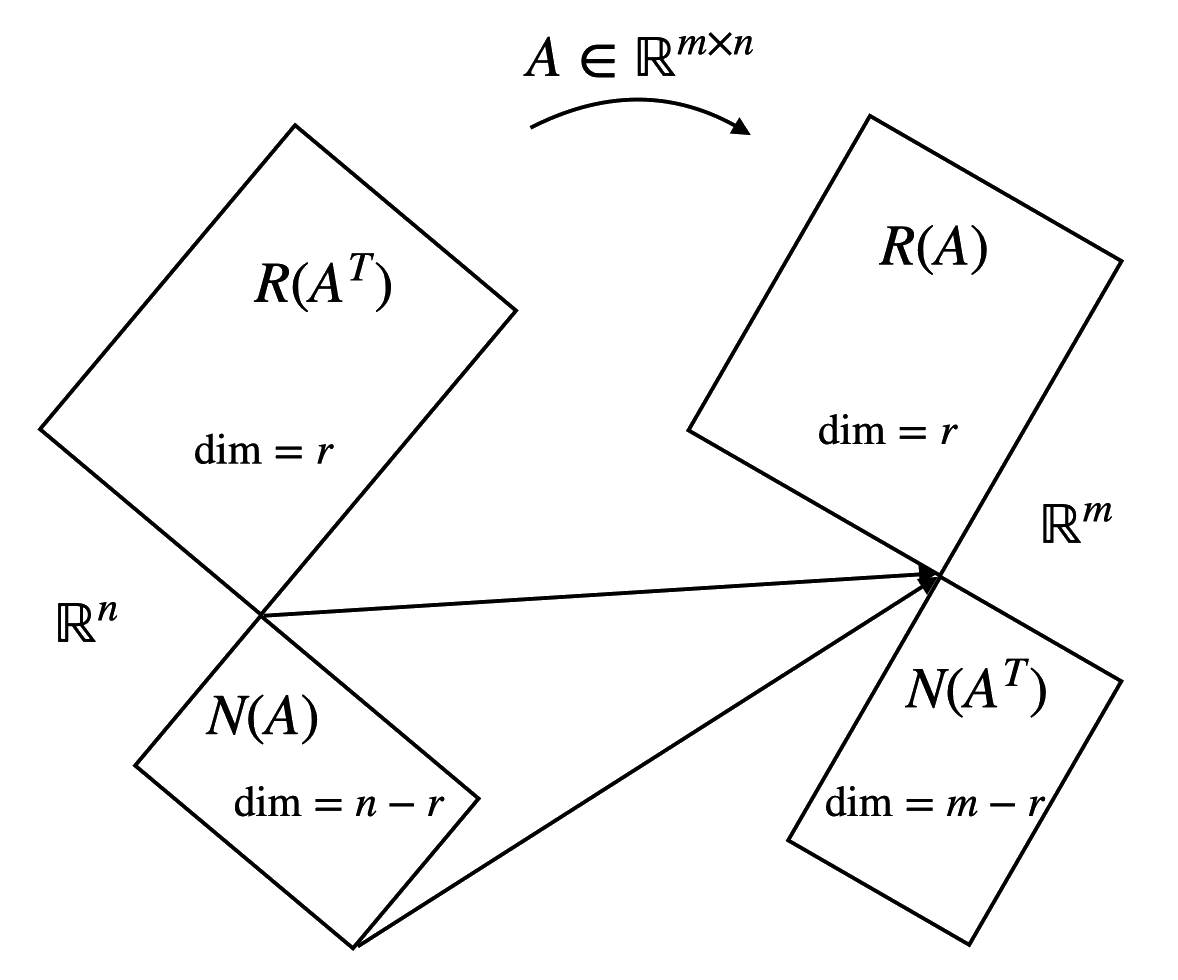
\includegraphics[width=0.55\linewidth]{figs/space.png}
\end{figure}
\end{remark}


\subsection{线性映射,线性变换及其矩阵表示}

表示是什么?表示究其本质来说是一种映射,它把我们不熟悉或抽象的事物映射为我们熟知或具体的事物。例如:抽象的线性空间在一个基下可表示为实或复的列向量空间。同样地,线性空间之间的线性映射都可以表示为矩阵,这正是矩阵的代数本质所在。这就是本节所研究的内容。


\begin{definition}[线性映射]
设有数域相同的线性空间 $X$ 到线性空间 $Y$ 的映射 $T$,若满足:
\begin{itemize}
    \item $T(x+y)=T(x)+T(y)$
    \item $T(kx)=kT(x)$
\end{itemize}
则称 $T$ 为 $X$ 到 $Y$ 的线性映射。
\end{definition}

\begin{definition}[线性映射的矩阵表示]
\label{def:matrixrepr}
设有 $m$ 维线性空间 $W$ 和 $n$ 维线性空间 $V$,$X=(x_1,\ldots,x_m)$,$Y=(y_1,\ldots,y_n)$ 分别是 $W,V$ 的基。$X$ 被 $T$ 映射到 $V$ 中后可以由 $Y$ 线性表示,即:
\[
\begin{cases}
Tx_1=a_{11}y_1+\cdots+a_{n1}y_n\\
\quad\vdots\\
Tx_m=a_{1m}y_1+\cdots+a_{nm}y_n\\
\end{cases}
\]
写作矩阵形式为:
\[
TX=Y
\underbrace{\begin{bmatrix}
a_{11}&\cdots&a_{1m}\\
\vdots&\ddots&\vdots\\
a_{n1}&\cdots&a_{nm}\\
\end{bmatrix}}_A
\]
称 $A\in\mathbb R^{n\times m}$ 为 $T$ 在基 $X,Y$ 下的矩阵表示。
\end{definition}

\begin{remark}
式 $TX=YA$ 非常重要,日后将经常使用。
\end{remark}

\begin{theorem}[向量在不同基下的表示坐标的关系]
设向量 $x\in W$ 在 $X$ 下的坐标表示为 $\xi$,$Tx\in V$ 在 $Y$ 下的坐标表示为 $\eta$,$T$ 在 $X,Y$ 下的矩阵表示为 $A$,那么有 $\eta=A\xi$. 可视化如下:
\[
\begin{array}{ccccccc}
    T: & x   & \mapsto & y    & = & T & x   \\
    \downarrow & \downarrow & & \downarrow & & \downarrow & \downarrow \\
    A: & \xi & \mapsto & \eta & = & A & \xi
\end{array}
\]
\end{theorem}
\begin{proof}
$Tx=T(X\xi)=(TX)\xi=(YA)\xi=Y(A\xi)=Y\eta\implies \eta=A\xi$
\end{proof}

从定义 \ref{def:matrixrepr} 可以看见,\textbf{线性映射的矩阵表示依赖于基的选取},即 $A=\sigma(T;X,Y)$. 既然如此,一个自然的问题就是,同一个线性映射在不同基下的矩阵表示有什么关系呢?

\begin{theorem}[同一个线性映射在不同基下的矩阵表示的关系]
设 $W,V$ 空间中的另一组基为 $X',Y'$,且 $X'=XC,\,Y'=YD$,其中 $C,D$ 为过渡矩阵(因而可逆),那么有 $A'=D^{-1}AC$. 
注意其中 $D\in\mathbb R^{n\times n},\,A\in\mathbb R^{n\times m},\,C\in\mathbb R^{m\times m}$.
\end{theorem}
\begin{proof}
$TX'=T(XC)=(TX)C=(YA)C=Y'D^{-1}AC=Y'A'\implies A'=D^{-1}AC$
\end{proof}

\begin{definition}[线性映射的复合]
设 $S:W\to V,\,T: V\to U$,定义它们的复合为 $(T\circ S)(x)=T(S(x))$. 显然,线性映射的复合仍为线性映射。
\end{definition}

\begin{theorem}[复合线性映射的矩阵表示]
设 $W,V,U$ 下各有基 $X,Y,Z$,在这些基下 $S,T$ 的矩阵表示分别为:$A=\sigma(S;X,Y)$,$B=\sigma(T;Y,Z)$,则复合映射 $T\circ S$ 的矩阵表示为 $BA$.
\end{theorem}
\begin{proof}
$(T\circ S)(X)=T(S(X))=T(YA)=(TY)A=(ZB)A=Z(BA)$
\end{proof}

\begin{com}
可以看见 $BA$ 只与 $X,Z$ 有关,与 $Y$ 无关,即 $BA=\sigma(T\circ S;X,Z)$. 事实上,我们可以选取 $V$ 的另一组基证明这一点:设 $Y'$ 也是 $V$ 的基且 $Y=Y'C$,那么:
\begin{align*}
    &SX=YA=(Y'C)A=Y'(CA)=Y'A'\implies CA=A'\\
    &TY=T(Y'C)=(TY')C=(ZB')C=Z(B'C)=ZB\implies B'C=B
\end{align*}
因此 $BA=(B'C)A=B'(CA)=B'A'$.
\end{com}

\begin{theorem}
设$T$为线性空间$W$到线性空间$V$的线性映射,则 $W$ 内的线性子空间$W_1$在$V$中的象$V_1$为$V$的线性子空间。反之,$V$ 中的线性子空间 $V_1$ 的逆象 $T^{-1}(V_1)=\{x\mid \exists y\in V_1,\,y=Tx\}$ 也是 $W$ 中的子空间。
\end{theorem}
\begin{proof}
利用子空间的定义易证(验证是否满足两条要求即可)。
\end{proof}

\begin{theorem}
设$T$为线性空间$W$到线性空间$V$的线性映射,$W_1,W_2$为$W$内的子空间,则:
\begin{itemize}
    \item $T(W_1+W_2)=T(W_1)+T(W_2)$
    \item $T(W_1\cap W_2)\subset T(W_1)\cap T(W_2)$
\end{itemize}
\end{theorem}

\begin{definition}[线性映射的值域和核]
设有线性映射 $T:W\to V$,则有与矩阵类似的定义:
\begin{itemize}
    \item 值域:$R(T)=\{y\in V\mid y=Tx,\forall x\in W\}$
    \item 核:$N(T)=\{x\mid Tx=0,x\in W\}$
    \item 秩:$\dim(R(T))$
    \item 亏度:$\dim(N(T))$
\end{itemize}
\end{definition}

\begin{theorem}[线性映射的维数公式]
设有线性映射 $T:W\to V$,则:
\[\dim(R(T))+\dim(N(T))=\dim(W)\]
\end{theorem}
\begin{proof}
可以用基扩充的方式来证明,与矩阵的维数公式类似,此处略去。
\end{proof}

\begin{theorem}[线性映射构成的空间]
设有线性映射 $T_1,T_2: W\to V$,定义加法和数乘如下:
\begin{itemize}
    \item 加法:$(T_1+T_2)(x)=T_1(x)+T_2(x)$
    \item 数乘:$(kT_1)(x)=k(T_1(x))$
\end{itemize}
则 $W$ 到 $V$ 的线性映射全体在上述加法和数乘下构成一个线性空间。
\end{theorem}

\begin{remark}
根据上文的讨论,我们知道线性映射在给定基后可以用矩阵表示。因此\textbf{我们可以借助矩阵来研究线性映射的性质,或借助线性映射来研究矩阵的性质}。例如下面的定理。
\end{remark}

\begin{theorem}[线性映射复合的维数公式]
设 $A\in\mathbb C^{m\times n}$,$B\in\mathbb C^{n\times p}$,则:
\begin{align*}
    &\dim(N(AB))=\dim(N(B))+\dim(N(A)\cap R(B))\\
    &\dim(R(AB))=\dim(R(B))-\dim(N(A)\cap R(B))
\end{align*}
\end{theorem}
\begin{proof}
首先证明第一个式子,依旧采用基扩充的思路。存在一组线性无关的 $x_1,\ldots,x_r\in\mathbb C^p$ 使得 $(Bx_1,\ldots,Bx_r)$ 为 $N(A)\cap R(B)$ 的一个基,再取 $N(B)$ 的一个基 $(y_1,\ldots,y_s)$,则只需要证明 $(x_1,\ldots,x_r,y_1,\ldots,y_s)$ 构成 $N(AB)$ 的一个基即可。

首先证明线性无关。由于 $(x_1,\ldots,x_r)$ 线性无关,$(y_1,\ldots,y_s)$ 线性无关,因此只需要证明 $y_j\ (j=1,\ldots,s)$ 与 $(x_1,\ldots,x_r)$ 线性无关即可。这是容易的,因为 $y_j\in N(B),\,x_i\in R(B)$,而 $N(B)\cap R(B)=\{0\}$.

其次,任取 $z\in N(AB)$,那么 $ABz=0$.  当 $Bz=0$ 时,$z\in N(B)$,可以被 $(y_1,\ldots,y_s)$ 线性表示;当 $Bz\neq 0$ 时,$Bz\in N(A)\cap R(B)$,因此 $Bz$ 可以被 $(Bx_1,\ldots,Bx_r)$ 线性表示,即:
\[
    Bz=\sum_{i=1}^r a_i Bx_i\implies B\left(z-\sum_{i=1}^ra_ix_i\right)=0
\]
但由于 $z,x_i\notin N(B)$,所以只能是括号内为零,即 $z$ 可以被 $(x_1,\ldots,x_r)$ 线性表示。

对于第二个式子,可以类似地采用基扩充的思路证明,这里选择另一种方法。利用上一条定理的结论,结合:
\[
    \dim(R(AB))+\dim(N(AB))=\dim(R(B))+\dim(N(B))=p
\]
即可推出结论。
\end{proof}

\begin{remark}
将矩阵 $A,B$ 看作线性映射,那么这两条定理可以直观地按下图理解:
\begin{figure}[H]
    \centering
    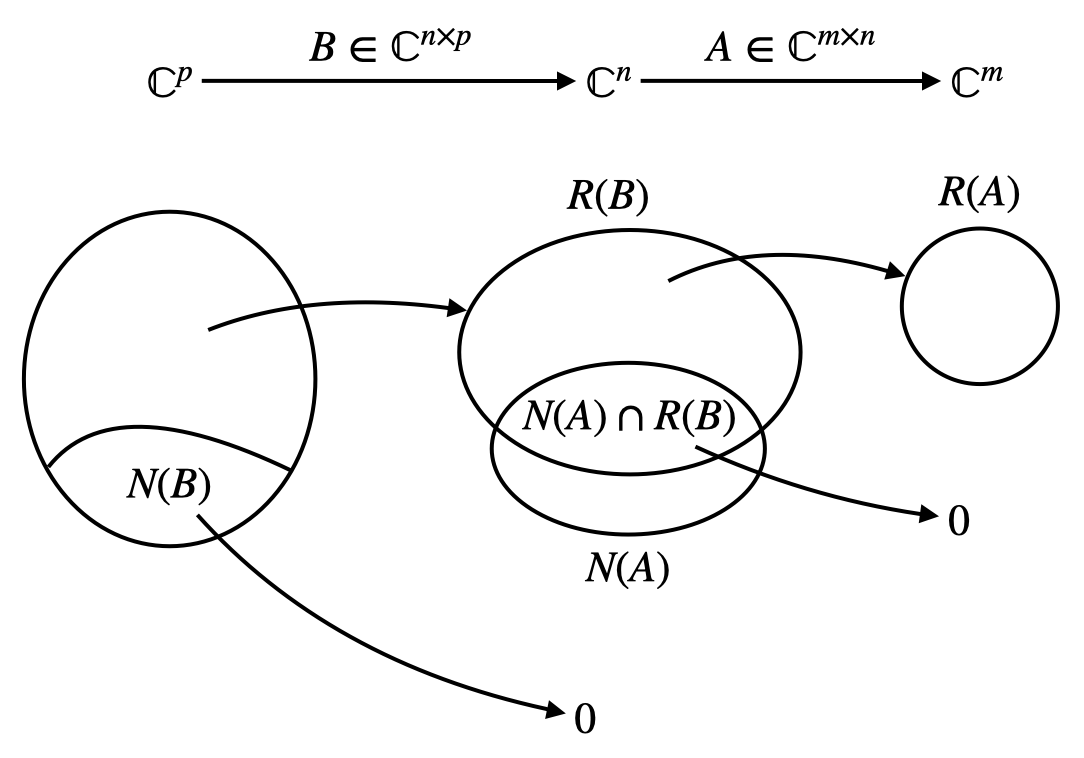
\includegraphics[width=0.55\linewidth]{figs/mapping.png}
\end{figure}
\begin{itemize}
    \item $N(AB)$ 包含被 $B$ 映射到了 $0$ 的部分和没被 $B$ 映射到 $0$、但被 $A$ 映射到 $0$ 的部分。
    \item $R(AB)$ 是没有被 $B$ 映射到 $0$ 的部分中,也没有被 $A$ 映射到 $0$ 的部分。
\end{itemize}
\end{remark}

\begin{corollary}
设 $A\in\mathbb C^{m\times n}$,$B\in\mathbb C^{n\times p}$,$C\in\mathbb C^{p\times q}$,则:
\begin{align*}
    &\text{rank}(A)+\text{rank}(B)-n\leq \text{rank}(AB)\\
    &\dim(R(AB))+\dim(R(BC))-\dim(R(B))\leq \dim(R(ABC))
\end{align*}
\end{corollary}
\begin{proof}
1) 由于:
\[
    \dim(R(B))-\dim(R(AB))=\dim(N(A)\cap R(B))\leq\dim(N(A))=n-\dim(R(A))
\]
等号成立当且仅当 $N(A)\subset R(B)$. 所以:
\[
    \dim(R(A))+\dim(R(B))-n\leq\dim(R(AB))
\]
即 $\text{rank}(A)+\text{rank}(B)-n\leq \text{rank}(AB)$.

2) 类似地,由于:
\begin{align*}
    \dim(R(BC))-\dim(R(ABC))&=\dim(N(A)\cap R(BC))\\
    &\leq \dim(N(A)\cap R(B))=\dim(R(B))-\dim(R(AB))
\end{align*}
所以:
\[
    \dim(R(AB))+\dim(R(BC))-\dim(R(B))\leq \dim(R(ABC))
\]
等号成立的条件为 $N(A)\cap R(BC)=N(A)\cap R(B)$.
\end{proof}

\begin{definition}[线性变换]
线性变换是从一个线性空间映射到它本身的线性映射,即 $T:W\to W$.
\end{definition}

\begin{definition}[线性变换的矩阵表示]
由于线性变换只涉及一个空间,所以当我们讨论线性映射的矩阵表示时,只需选择一个基 $X$,即:
\[TX=XA\]
当然,我们也可以选择两个不同的基 $X,Y$,这时相当于把线性变换依旧视作线性映射。本课程以后提到线性变换时都只选择一个基。
\end{definition}

与线性映射在不同基下有不同的矩阵表示类似,线性变换在不同基下也有着不同的矩阵表示,这引出了相似矩阵的定义。

\begin{theorem}[线性变换在不同基下的矩阵表示]
\label{thm:sim-trans}
设线性变换 $T$ 在基 $X$ 下的矩阵表示为 $A$,在基 $X'$ 下的矩阵表示为 $A'$,且两个基之间的关系为:$X'=XC$,那么 $A'=C^{-1}AC$.
\end{theorem}
\begin{proof}
\[
TX'=T(XC)=(TX)C=(XA)C=X(AC)=X'C^{-1}AC=X'A'\implies A'=C^{-1}AC
\]
\end{proof}

\begin{definition}[相似矩阵]
设 $A,A'$ 为 $n$ 阶矩阵,若存在可逆矩阵 $C$ 使得:
\[A'=C^{-1}AC\]
则称 $A$ 与 $A'$ 是相似的。
\end{definition}

\begin{property}
矩阵相似关系为等价关系,即满足:
\begin{itemize}
    \item 自反性:$A$ 和 $A$ 相似;
    \item 对称性:若 $A$ 和 $B$ 相似,则 $B$ 和 $A$ 相似;
    \item 传递性:若 $A$ 和 $B$ 相似,$B$ 和 $C$ 相似,则 $A$ 和 $C$ 相似。
\end{itemize}
\end{property}

\begin{remark}
可以看见,\textbf{相似矩阵本质上是同一个线性变换在不同基下的表示}。因此,\textbf{相似等价意义下矩阵具有的性质本质上是对应线性变换的性质}。例如,我们即将看见相似矩阵的行列式相同,本质这是因为行列式对应着线性变换对原空间的单位超立方体变换后的体积。
\end{remark}

\begin{definition}[线性变换的多项式]
记 $T^2$ 表示复合变换 $T\circ T$;类似地,记 $T^k=T^{k-1}\circ T$. 进一步地,记线性变换的多项式为 $f(T)=a_0T^m+a_1T^{m-1}+\cdots+a_{m-1}T+a_mI$.
\end{definition}

\begin{theorem}[线性变换的多项式的矩阵表示]
若 $T$ 的矩阵表示为 $A$,那么 $T^k$ 的矩阵表示为 $A^k$;进一步地,多项式 $f(T)$ 的矩阵表示为 $f(A)$.
\end{theorem}

上面定义了线性变换的多项式,自然地,我们思考能否定义线性变换的一般函数,例如 $\exp(T)$ 或 $\sin(T)$?不过,这个问题需要 Hamilton-Cayley 定理 \ref{thm:Hamilton-Cayley} 和第三章的相关知识,我们将在 \ref{sec:3-matrix-function} 节中给出答案。


\subsection{线性变换的表示}

由于线性变换在不同基下的矩阵表示不相同,那么一个很自然的问题就是,怎样选择特殊的基使得给定线性变换在这个基下的表示矩阵尽可能简单?换个说法,由于同一线性变换的不同矩阵表示之间是相似关系,这个问题等价于,如何找到一个形式尽可能简单的矩阵使之相似于给定矩阵——这就是本节的终极目标 Jordan 标准形。不过在此之前,我们首先要介绍有关特征值与特征向量的基础知识。

\begin{definition}[矩阵的特征值与特征向量]
设 $A$ 为 $n$ 阶矩阵,若存在非零向量 $x$ 和数 $\lambda$ 满足 $Ax=\lambda x$,则称 $\lambda$ 为矩阵 $A$ 的特征值,$x$ 为属于 $\lambda$ 的特征向量。
\end{definition}

\begin{theorem}
$n$ 阶矩阵 $A$ 奇异当且仅当 $0$ 是 $A$ 的特征值。
\end{theorem}
\begin{proof}
$n$ 阶矩阵 $A$ 奇异 $\iff$ 存在 $x\neq0$ 使得 $Ax=0$ $\iff$ 存在 $x\neq0$ 使得 $Ax=0\cdot x$ $\iff$ $0$ 是 $A$ 的特征值。
\end{proof}

根据特征值的定义,若 $\lambda,\,x\neq0$ 是矩阵 $A$ 的特征值和对应特征向量,则有 $Ax=\lambda x$,即 $(\lambda I-A)x=0$. 由于 $x\neq 0$,因此该方程有解当且仅当 $\lambda I-A$ 奇异,即 $\det(\lambda I-A)=0$. 我们据此定义特征多项式与特征方程。

\begin{definition}[特征多项式,特征方程]
设 $A$ 为一个 $n$ 阶矩阵,称多项式 $\varphi(\lambda)=\det(\lambda I-A)$ 为矩阵 $A$ 的特征多项式,方程 $\det(\lambda I-A)=0$ 为矩阵 $A$ 的特征方程。
\end{definition}

设 $\lambda_0$ 是特征多项式 $\varphi(\lambda)$ 的零点,那么相应方程 $(\lambda_0I-A)x=0$ 就有非零解,不妨设为 $x_0\neq0$,于是有 $Ax_0=\lambda_0x_0$,即 $\lambda_0$ 是矩阵 $A$ 的特征值,$x_0$ 是相应的特征向量。因此我们有结论:特征多项式 $\varphi(\lambda)$ 的零点就是矩阵 $A$ 的特征值。反之,根据定义,矩阵 $A$ 的特征值显然是特征多项式的零点。又根据\textbf{代数基本定理},$n$ 阶多项式在复数域中必有 $n$ 个零点(可能重合),因此为了方便起见,我们给特征值的重数做出以下定义。

\begin{definition}[代数重数]
设 $A$ 为一个 $n$ 阶矩阵,$\lambda_0$ 为其一个特征值,称 $\lambda_0$ 作为特征多项式 $\varphi(\lambda)$ 的零点的重数为它的代数重数。
\end{definition}

有了代数重数的定义,我们就可以直接断言:\textbf{任意 $n$ 阶矩阵在复数域中恰有 $n$ 个特征值(可能重复)}。设这 $n$ 个特征值为 $\lambda_1,\lambda_2,\ldots,\lambda_n$(重复特征值重复写出),那么特征多项式也可以写作:
\[
    \varphi(\lambda)=(\lambda-\lambda_1)(\lambda-\lambda_2)\cdots(\lambda-\lambda_n)
\]
基于此,通过探究特征多项式根与系数的关系,我们可以得到下述常用结论。

\begin{theorem}[迹与特征值,行列式与特征值]
\ 

1) 矩阵 $A$ 的迹等于 $A$ 的所有特征值之和;

2) 矩阵 $A$ 的行列式等于 $A$ 的所有特征值之积。
\end{theorem}
\begin{proof}
设矩阵 $A$ 的特征值为 $\lambda_1,\lambda_2,\ldots,\lambda_n$,则特征多项式可写作:
\begin{align*}
    \varphi(\lambda)&=(\lambda-\lambda_1)(\lambda-\lambda_2)\cdots(\lambda-\lambda_n)\\
    &=\lambda^n-(\lambda_1+\lambda_2+\cdots+\lambda_n)\lambda^{n-1}+\cdots+(-1)^n\lambda_1\lambda_2\cdots\lambda_n
\end{align*}
另一方面,根据定义:
\[
    \varphi(\lambda)=\det(\lambda I-A)=
    \begin{vmatrix}
    \lambda-a_{11}&-a_{12}&\cdots&-a_{1n}\\
    -a_{21}&\lambda-a_{22}&\cdots&-a_{2n}\\
    \vdots&\vdots&\ddots&\vdots\\
    -a_{n1}&-a_{n2}&\cdots&\lambda-a_{nn}
    \end{vmatrix}
\]
将行列式按第一行展开,可以发现含有 $\lambda^n$ 和 $\lambda^{n-1}$ 的只有一项:
\[
    (\lambda-a_{11})(\lambda-a_{22})\cdots(\lambda-a_{nn})
\]
这是因为其他项最高只到 $\lambda^{n-2}$. 因此,对比二式中 $\lambda^{n-1}$ 的系数可知:
\[
    \lambda_1+\lambda_2+\cdots+\lambda_n=a_{11}+a_{22}+\cdots+a_{nn}=\text{tr}(A)
\]
即矩阵 $A$ 的迹等于 $A$ 的所有特征值之和。另外,在特征多项式中代入 $\lambda=0$,得:
\[
    \det(-A)=(-1)^n\det(A)=(-1)^n\lambda_1\lambda_2\cdots\lambda_n
\]
因此有:
\[
    \det(A)=\lambda_1\lambda_2\cdots\lambda_n
\]
即矩阵 $A$ 的行列式等于 $A$ 的所有特征值之积。
\end{proof}

\begin{theorem}
\label{thm:sim-eigen}
相似矩阵有相同的特征多项式。
\end{theorem}
\begin{proof}
设 $A$ 与 $B$ 相似,则存在可逆矩阵 $P$ 使得 $P^{-1}AP=B$,于是:
\begin{align*}
    \det(\lambda I-B)&=\det(P^{-1}(\lambda I)P-P^{-1}AP)=\det(P^{-1}(\lambda I-A)P)\\
    &=\det(P^{-1})\det(\lambda I-A)\det(P)=\det(\lambda I-A)
\end{align*}
即 $A$ 与 $B$ 的特征多项式相同。
\end{proof}

\begin{corollary}
相似矩阵的特征值相同、迹相同、行列式相同。
\end{corollary}

\begin{theorem}[$AB$ 和 $BA$ 有相同的非零特征值]
\label{thm:eigen-ab-ba}
设 $A\in\mathbb F^{m\times n},B\in\mathbb F^{n\times m}$,记 $AB$ 的特征多项式为 $\varphi_{AB}(\lambda)$,$BA$ 的特征多项式为 $\varphi_{BA}(\lambda)$,则:
\[
    \lambda^n\varphi_{AB}(\lambda)=\lambda^m\varphi_{BA}(\lambda)
\]
即 $AB$ 和 $BA$ 有相同的非零特征值。
\end{theorem}
\begin{proof}
由于:
\[
    \begin{bmatrix}I_m&0\\-B&I_n\end{bmatrix}\begin{bmatrix}I_m&A\\0&\lambda I_n\end{bmatrix}\begin{bmatrix}\lambda I_m-AB&0\\B&I_n\end{bmatrix}=\begin{bmatrix}I_m&A\\0&\lambda I_n-BA\end{bmatrix}
\]
等式两边取行列式即得证。
\end{proof}
\begin{proof}[更直接的证明方法]
设 $\lambda,x$ 为 $AB$ 的特征值和特征向量,即 $ABx=\lambda x$,那么左乘 $B$ 得到:\[(BA)(Bx)=\lambda (Bx)\]
也就是说 $\lambda$ 和 $Bx$ 是 $BA$ 的特征值和特征向量。
\end{proof}

\begin{corollary}
设 $A\in\mathbb F^{m\times n},B\in\mathbb F^{n\times m}$,则 $\text{tr}(AB)=\text{tr}(BA)$,$\det(AB)=\det(BA)$.
\end{corollary}

\begin{corollary}
\label{cor:trace}
设 $A\in\mathbb F^{m\times n},B\in\mathbb F^{n\times p},C\in\mathbb F^{p\times m}$,则 $\text{tr}(ABC)=\text{tr}(BCA)=\text{tr}(CAB)$. 以此类推,对于更多矩阵相乘的情形有类似的轮换性质。
\end{corollary}

\begin{theorem}[特征向量的线性无关性]
\label{thm:eigenind}
设 $A$ 为矩阵,$\lambda_1,\ldots,\lambda_s$ 为 $A$ 的\textbf{互不相同}的特征值,$x_1,\ldots,x_s$ 是分别属于这些特征值的特征向量,那么 $x_1,\ldots,x_s$ 线性无关。
\end{theorem}
\begin{proof}
考虑数学归纳法。首先,单个特征向量 $x_1$ 线性无关;其次,假设 $x_1,\ldots,x_{s-1}$ 线性无关,设 $\sum_{i=1}^s k_ix_i=0$,用 $A$ 左乘上式得:
\[
    \sum_{i=1}^sk_iAx_i=\sum_{i=1}^sk_i\lambda_ix_i=0
\]
根据上面两个式子消去 $x_s$,得:
\[
    \sum_{i=1}^{s-1}k_i(\lambda_i-\lambda_s)x_i=0
\]
根据归纳假设,有 $k_i(\lambda_i-\lambda_s)=0$;又特征值互不相同,故 $k_i=0\ (i=1,\ldots,s-1)$. 进而 $k_s=0$.
\end{proof}

\begin{theorem}[特征向量的线性无关性-续]
设 $A$ 为矩阵,$\lambda_1,\ldots,\lambda_k$ 为 $A$ 的\textbf{互不相同}的特征值,$x_{i1},\ldots,x_{ir_i}$ 是属于 $\lambda_i$ 的线性无关特征向量,那么 $x_{11},\ldots,x_{1r_1},\ldots,x_{k1},\ldots,x_{kr_k}$ 线性无关。
\end{theorem}
\begin{proof}
设 $\sum_{i=1}^k\sum_{j=1}^{r_i}k_{ij}x_{ij}=0$,记 $x_i=\sum_{j=1}^{r_i}k_{ij}x_{ij}$,左乘 $A$ 得:
\[
    Ax_i=\sum_{j=1}^{r_i}k_{ij}Ax_{ij}=\sum_{j=1}^{r_i}k_{ij}\lambda_ix_{ij}=\lambda_ix_i
\]
假设 $x_i\neq0$,则 $x_i$ 是 $A$ 属于 $\lambda_i$ 的特征向量,又由于 $\sum_{i=1}^kx_i=0$,根据定理 \ref{thm:eigenind} 知 $x_i=0$,矛盾,因此只能有 $x_i=0$. 由线性无关性可知,所有的 $k_{ij}=0$.
\end{proof}

\begin{theorem}
\label{thm:anysimilar}
任意 $n$ 阶矩阵都与一个上三角矩阵相似。
\end{theorem}
\begin{proof}
考虑数学归纳法。设 $A$ 是一个 $n$ 阶矩阵,$x_1$ 为 $A$ 的特征值 $\lambda$ 对应的特征向量。将 $x_1$ 扩充为 $\mathbb C^n$ 的一个基 $(x_1,\ldots,x_n)$,那么 $Ax_i$ 都可以被这个基线性表示:
\[
\begin{cases}
Ax_1=b_{11}x_1+b_{21}x_2+\cdots+b_{n1}x_n=\lambda x_1\\
Ax_2=b_{12}x_1+b_{22}x_2+\cdots+b_{n2}x_n\\
\quad\vdots\\
Ax_n=b_{1n}x_1+b_{2n}x_2+\cdots+b_{nn}x_n
\end{cases}
\]
写作矩阵形式:
\[
AX=XB=X\begin{bmatrix}\lambda&b_{12}&\cdots&b_{1n}\\0&b_{22}&\cdots&b_{2n}\\\vdots&\vdots&\ddots&\vdots\\0&b_{n2}&\cdots&b_{nn}\end{bmatrix}=X\begin{bmatrix}\lambda&\alpha^T\\0&B_1\end{bmatrix}
\]
根据归纳假设,设 $B_1=QUQ^{-1}$ 且 $U$ 是上三角矩阵,那么:
\[
AX=X\begin{bmatrix}\lambda&\alpha^T\\0&QUQ^{-1}\end{bmatrix}=X\begin{bmatrix}1&0\\0&Q\end{bmatrix}\begin{bmatrix}\lambda&\alpha^T\\0&U\end{bmatrix}\begin{bmatrix}1&0\\0&Q^{-1}\end{bmatrix}
\]
所以 $A$ 相似于上三角矩阵 $\begin{bmatrix}\lambda&\alpha^T\\0&U\end{bmatrix}$.
\end{proof}

\begin{definition}[零化多项式]
设 $A$ 是一个 $n$ 阶矩阵,若多项式 $f(x)$ 使得 $f(A)=0$,则称 $f(x)$ 为矩阵 $A$ 的一个零化多项式。
\end{definition}

\begin{theorem}[Hamilton-Cayley 定理]
\label{thm:Hamilton-Cayley}
设 $A$ 是一个 $n$ 阶矩阵,则 $A$ 的特征多项式是其零化多项式。形式化地说,设:
\[
\varphi(\lambda)=\det(\lambda I-A)=\lambda^n+a_1\lambda^{n-1}+\cdots+a_{n-1}\lambda+a_n
\]
则:
\[
\varphi(A)=A^n+a_1A^{n-1}+\cdots+a_{n-1}A+a_nI_n=0
\]
\end{theorem}

\begin{proof}
考虑数学归纳法。首先,当 $n=1$ 时,定理显然成立;其次,设定理对 $n-1$ 阶矩阵成立,下面证明对 $n$ 阶矩阵依然成立。设 $A$ 的 $n$ 个特征值为 $\lambda_1,\ldots,\lambda_n$,根据定理 \ref{thm:anysimilar} 的证明过程可知,$A$ 相似于:
\[R=\begin{bmatrix}\lambda_1&\alpha^T\\0&U\end{bmatrix}\]
即存在可逆矩阵 $P$ 使得 $A=P^{-1}RP$,其中 $U$ 为上三角矩阵。由于相似矩阵有相同的特征值,所以 $\lambda_1,\ldots,\lambda_n$ 也是 $R$ 的特征值。容易知道 $\lambda_2,\ldots,\lambda_n$ 是 $U$ 的特征值。又因为:
\[
\varphi(A)=\varphi(P^{-1}RP)=\sum_{i=0}^n a_{n-i}(P^{-1}RP)^i=\sum_{i=0}^n a_{n-i}P^{-1}R^iP=P^{-1}\varphi(R)P
\]
所以要证明 $\varphi(A)=0$,只需要证明 $\varphi(R)=0$.
\begin{align*}
\varphi(R)&=(R-\lambda_1I_n)\cdots(R-\lambda_n I_n)\\
&=\begin{bmatrix}\lambda_1-\lambda_1&\alpha^T\\0&U-\lambda_1I_{n-1}\end{bmatrix}\cdots\begin{bmatrix}\lambda_n-\lambda_1&\alpha^T\\0&U-\lambda_nI_{n-1}\end{bmatrix}\\
&=\begin{bmatrix}0&\alpha^T\\0&U-\lambda_1I_{n-1}\end{bmatrix}\begin{bmatrix}\prod_{j=2}^n(\lambda_j-\lambda_1)&\beta^T\\0&\prod_{j=2}^n(U-\lambda_jI_{n-1})\end{bmatrix}\\
&=\begin{bmatrix}0&0\\0&(U-\lambda_1 I_{n-1})\prod_{j=2}^n(U-\lambda_jI_{n-1})\end{bmatrix}
\end{align*}
根据归纳假设,$\prod_{j=2}^n(U-\lambda_jI_{n-1})=0$,因此上式为 $0$.
\end{proof}

\begin{corollary}
对于 $n$ 阶矩阵 $A$,$\{A^n,A^{n-1},\ldots,A,I_n\}$ 线性相关。
\end{corollary}

\begin{corollary}
\label{cor:invpoly}
任何一个 $n$ 阶可逆矩阵 $A$ 的逆可表示为 $A$ 的次数不超过 $n-1$ 的多项式,即:
\[A^{-1}=g(A)=a_1A^{n-1}+a_2A^{n-2}+\cdots+a_{n-1}A+a_nI_n\]
\end{corollary}

\begin{definition}[最小多项式]
零化多项式中,称次数最低的首项系数为 1 的零化多项式 $m(\lambda)$ 为最小多项式。(注意这里 $\lambda$ 只是一个变量符号,不是特征值的意思)
\end{definition}

\begin{theorem}
\label{thm:minpoly}
最小多项式可以整除任意其他首项系数为 1 的零化多项式 $\psi(\lambda)$,且是唯一的。
\end{theorem}
\begin{proof}
作多项式除法:$\psi(\lambda)=m(\lambda)p(\lambda)+r(\lambda)$,其中 $r(\lambda)$ 的次数小于 $m(\lambda)$ 的次数。由于 $\psi(A)=m(A)=0$,故 $r(A)=0$,但由于 $m(\lambda)$ 是次数最小的零化多项式,所以只能是 $r(\lambda)=0$.  因此 $m(\lambda)\mid\psi(\lambda)$.
\end{proof}

\begin{theorem}
矩阵 $A$ 的最小多项式 $m(\lambda)$ 和特征多项式 $\varphi(\lambda)$ 零点相同(重数可以不同)。换句话说,$m(\lambda)$ 的零点就是特征值,只是与 $\varphi(\lambda)$ 的次数不同。
\end{theorem}
\begin{proof}
根据定理 \ref{thm:minpoly},$\varphi(\lambda)=m(\lambda)p(\lambda)$,所以 $m(\lambda)=0\implies \varphi(\lambda)=0$. 因此现在只需证明 $\varphi(\lambda)=0\implies m(\lambda)=0$.
设 $\varphi(\lambda_0)=0$,$A x_0=\lambda_0 x_0$,则 $m(A) x_0=m(\lambda_0) x_0=0$,由于 $x_0\neq 0$,所以 $m(\lambda_0)=0$.
\end{proof}

\begin{com}
显然,如果矩阵 $A$ 的最小多项式次数为 $m$,那么 $\{A^{m-1},\ldots,A,I_n\}$ 线性无关,但再加入一个 $A^m$ 就线性相关了。
\end{com}

本节至此我们都是站在矩阵的角度分析其特征值和特征向量,而前文我们提到过,借助线性变换来研究矩阵是非常重要的手段。基于这种思想,下面我们引入线性变换的特征值和特征向量,进而引入特征子空间和不变子空间的概念,最终得到著名的 Jordan 标准形。

\begin{definition}[线性变换的特征值与特征向量]
设 $T$ 是一个线性变换,若存在非零向量 $x$ 和数 $\lambda$ 满足 $Tx=\lambda x$,则称 $\lambda$ 为 $T$ 的特征值,$x$ 为属于 $\lambda$ 的特征向量。
\end{definition}

\begin{theorem}[线性变换的特征值和特征向量与矩阵的特征值和特征向量]
设 $X$ 为线性空间中的一个基,线性变换 $T$ 在该基下的矩阵表示为 $A$. 若 $\lambda$ 为 $T$ 的一个特征值,对应特征向量 $x$ 在基 $X$ 下的坐标表示为 $\xi$,则 $\lambda$ 是 $A$ 的特征值,$\xi$ 是对应的特征向量。
\end{theorem}
\begin{proof}
由题意有 $x=X\xi,\,TX=XA,\,Tx=\lambda x$,因此:
\[
    \begin{cases}
    Tx=T(X\xi)=(TX)\xi=XA\xi\\
    Tx=\lambda x=\lambda X\xi=X(\lambda\xi)
    \end{cases}\implies A\xi=\lambda\xi
\]
即 $\lambda$ 是 $A$ 的特征值,$\xi$ 是对应的特征向量。
\end{proof}

\begin{remark}
线性变换的特征值和其矩阵表示的特征值是一样的,而特征向量的关系就是在选取的那个基下的坐标关系。
\end{remark}

基于上述结论,我们发现矩阵的特征值在本质上其实是背后的线性变换的性质,于是前文定理 \ref{thm:sim-eigen} 所述的“相似矩阵有相同的特征值”有了更直观简单的解释:相似矩阵是同一个线性变换的不同矩阵表示,其特征值就是线性变换的特征值,因此显然都是相同的。

\begin{definition}[特征子空间]
设 $T$ 为线性变换,$\lambda_0$ 为 $T$ 的一个特征值,则称 $\lambda_0I-T$ 的核空间($I$ 表示恒等变换)为 $T$ 属于 $\lambda_0$ 的特征子空间:
\[V_{\lambda_0}=N((\lambda_0I-T))=\{x\mid(\lambda_0 I-T)x=0\}\]
\end{definition}

\begin{com}
根据定义,若 $x\in V_{\lambda_0}$,则 $x$ 是属于 $\lambda_0$ 的特征向量。
\end{com}

\begin{definition}[几何重数]
设 $T$ 为线性变换,$\lambda_0$ 为 $T$ 的一个特征值,称 $\dim V_{\lambda_0}$ 为它的几何重数。
\end{definition}

\begin{theorem}[代数重数 $\geq$ 几何重数]
设 $T$ 为线性空间 $V$ 上的线性变换,$\lambda_0$ 为 $T$ 的一个特征值,则其代数重数大于等于几何重数。
\end{theorem}
\begin{proof}
设几何重数 $\dim V_{\lambda_0}=q$,取 $V_{\lambda_0}$ 的基 $x_1,\ldots,x_q$,将其扩充为 $V$ 的基 $x_1,\ldots,x_q,\ldots,x_n$. 由于对 $i=1,2,\ldots,q$,有 $Tx_i=\lambda_0x_i$,因此 $T$ 在基 $x_1,\ldots,x_q,\ldots,x_n$ 下的矩阵表示为:
\[
    A=\left[\begin{array}{ccc:ccc}
    \lambda_0 & \cdots & 0         & &        & \\
    \vdots    & \ddots & \vdots    & & A_{12} & \\
    0         & \cdots & \lambda_0 & &        & \\ \hdashline
              &        &           & &        & \\
              & O      &           & & A_{22} & \\
              &        &           & &        & \\
    \end{array}\right]
\]
于是特征多项式为:
\[
    \varphi(\lambda)=\det(\lambda I-A)=(\lambda-\lambda_0)^q\det(\lambda I_{n-q}-A_{22})
\]
故代数重数至少为 $q$.
\end{proof}

\begin{definition}[不变子空间]
若线性空间 $V$ 的线性子空间 $V_1$ 对线性变换 $T$ 保持不变,即:$\forall x\in V_1$,有 $Tx\in V_1$,则称 $V_1$ 是 $T$ 的不变子空间。这时 $T$ 可以看作 $V_1$ 上的线性变换,称为 $T$ 在 $V_1$ 上的限制 $T\vert V_1$.  但值得注意的是,$T$ 和 $T\vert V_1$ 是不同的线性变换(它们的输入维度都不同)。
\end{definition}
\begin{figure}[H]
    \centering
    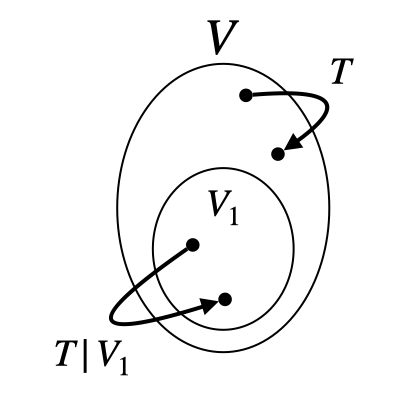
\includegraphics[width=0.2\linewidth]{figs/TV1.png}
\end{figure}

\begin{property}
不变子空间的和与交也是不变子空间。
\end{property}
\begin{proof}
设 $V_1,V_2$ 都是 $T$ 的不变子空间,则对于 $z\in V_1+V_2$,存在 $x\in V_1,\,y\in V_2$ 使得 $z=x+y$,并且 $Tx\in V_1,\,Ty\in V_2$,于是 $Tz=T(x+y)=Tx+Ty\in V_1+V_2$. 另外,对于 $z\in V_1\cap V_2$,由于 $Tz\in V_1,\,Tz\in V_2$,故 $Tz\in V_1\cap V_2$.
\end{proof}

\begin{property}
线性变换 $T$ 的值域 $R(T)$ 和核 $N(T)$ 都是 $T$ 的不变子空间。
\end{property}
\begin{proof}
对 $\forall x\in R(T)$,$Tx\in R(T)$,故 $R(T)$ 是 $T$ 的不变子空间;对于 $\forall x\in N(T)$,$Tx=0\in N(T)$,故 $N(T)$ 是 $T$ 的不变子空间。
\end{proof}

\begin{property}
设 $f(t)$ 为一多项式,则 $T$ 的不变子空间也是 $f(T)$ 的不变子空间。
\end{property}
\begin{proof}
设 $V_1$ 是 $T$ 的不变子空间,即 $\forall x\in V_1$,有 $Tx\in V_1$.  那么 $T^2x=T(Tx)\in V_1$,以此类推有 $f(T)(x)\in V_1$,即 $V_1$ 也是 $f(T)$ 的不变子空间。
\end{proof}

\begin{corollary}
若 $T$ 为可逆变换,则 $T$ 的不变子空间也是 $T^{-1}$ 的不变子空间。
\end{corollary}
\begin{proof}
根据推论 \ref{cor:invpoly},$T^{-1}$ 可写作 $T$ 的多项式,故可得结论。
\end{proof}

\begin{corollary}
特征子空间为不变子空间。
\end{corollary}
\begin{proof}
注意到 $\lambda I-T$ 是 $T$ 的多项式,故特征子空间 $V_\lambda=N(\lambda I-T)$ 为 $T$ 的不变子空间。
\end{proof}

\begin{theorem}
设 $T$ 为一个线性变换,$x$ 为 $T$ 的特征向量,则 $L(x)=\{z\mid z=kx,\,k\in \mathbb C\}$ 为 $T$ 的一维不变子空间。
\end{theorem}
\begin{proof}
对于 $z\in L(x)$,由于 $z$ 是 $T$ 的特征向量,因此存在 $\lambda\in\mathbb C$ 使得 $Tz=\lambda z\in L(x)$,故 $L(x)$ 是 $T$ 的不变子空间。
\end{proof}

基于不变子空间的概念,下面引入分块对角化与对角化。

\begin{theorem}[分块对角化]
\label{thm:blockdiag}
设 $T$ 是线性空间 $V^n$ 上的线性变换,假若 $V^n$ 可以分解为 $s$ 个 $T$ 的不变子空间的直和:
\[
    V^n=V_1\oplus\cdots\oplus V_s
\]
则 $T$ 在 $V^n$ 的某个基下的矩阵表示为分块对角矩阵:
\[
    A=\begin{bmatrix}A_1&&\\&\ddots&\\&&A_s\end{bmatrix}
\]
反之,若 $T$ 在基 $X=(X_1,\ldots,X_s)$ 下的矩阵表示为分块对角矩阵,则 $V^n$ 可分解为 $s$ 个不变子空间的直和。
\begin{figure}[H]
    \centering
    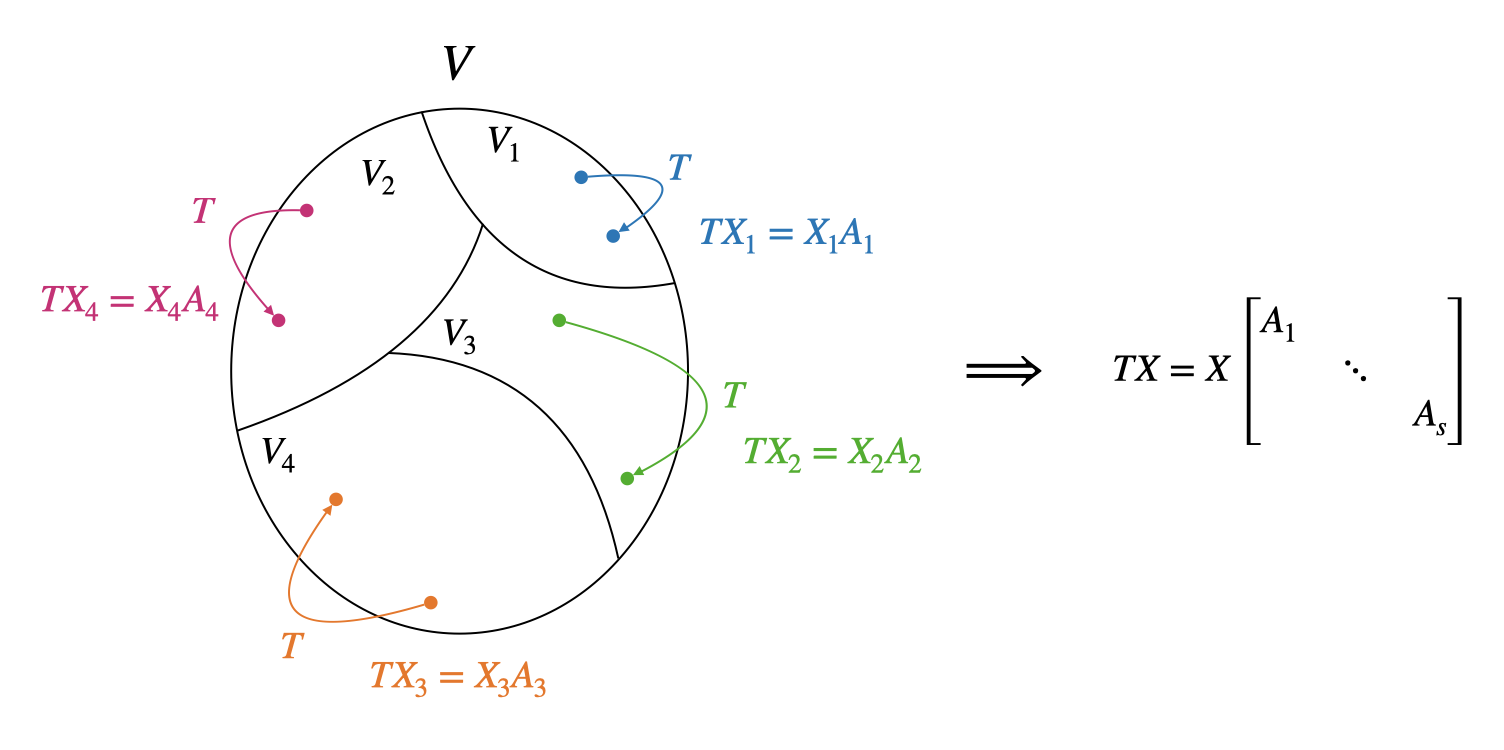
\includegraphics[width=0.8\linewidth]{figs/subspaces.png}
\end{figure}
\end{theorem}
\begin{proof}
设 $V^n$ 可以分解为 $s$ 个不变子空间的直和,在每个不变子空间 $V_i$ 中选取一个基 $X_i=(x_{i1},\ldots,x_{in_i}),\,(i=1,\ldots,s)$,将它们合并构成 $V^n$ 的基 $X=(X_1,\ldots,X_s)$,则显然 $T$ 在这个基下的矩阵表示为一个分块对角矩阵。反之,若 $T$ 在基 $X=(X_1,\ldots,X_s)$ 下的矩阵表示为分块对角矩阵,那么根据定义容易知道 $X_i$ 张成的子空间 $V_i$ 是 $T$ 的不变子空间,且 $V^n$ 是它们的直和。
\end{proof}

\begin{definition}[可对角化]
若线性空间 $V^n$ 上的线性变换 $T$ 在 $V^n$ 的某个基下的表示矩阵为对角阵,则称 $T$ 是可对角化的。
\end{definition}

\begin{theorem}[可对角化的充要条件]
设 $T$ 为 $V^n$ 上的线性变换,则:
\begin{align*}
    T \text{可对角化}&\iff \text{存在一组特征向量构成的基}\\
    &\iff \text{有}\ n\ \text{个线性无关的特征向量}\\
    &\iff \text{各个特征值的代数重数和几何重数相等}
\end{align*}
\end{theorem}
\begin{proof}
根据定义易知,每个特征向量张成的一维子空间都是一个一维不变子空间。因此,当 $T$ 有 $n$ 个线性无关的特征向量时(这些特征向量构成了一组基),$V^n$ 就可以写作这些特征向量分别张成的一维不变子空间的直和。于是根据定理 \ref{thm:blockdiag},$T$ 在这些特征向量构成的基下的矩阵表示为对角阵。
\end{proof}

\begin{corollary}[可对角化的充分条件]
若 $T$ 有 $n$ 个不同特征值,则 $T$ 可对角化。
\end{corollary}
\begin{proof}
根据定理 \ref{thm:eigenind} 可知 $T$ 有 $n$ 个线性无关的特征向量,因此 $T$ 可对角化。
\end{proof}

至此我们初步回答了本节开头提出的问题。如果线性变换存在一组特征向量构成的基,那么在这个基下它的表示矩阵就是我们所期望的最简单的对角阵形式。然而,并不是所有矩阵都有 $n$ 个线性无关的特征向量,所以现在我们必须回到分块对角化的形式上继续研究。注意分块对角化的前提假设是“空间可以分解为若干不变子空间的直和”,那这个假设是否总是成立呢?下面的定理告诉我们,这个假设不仅成立,而且这些不变子空间与特征值息息相关。

\begin{theorem}[基于不变特征子空间的直和分解]
\label{thm:directsum}
设 $T$ 是线性空间 $V^n$ 上的线性变换,任取 $V^n$ 的一个基,$T$ 在该基下的矩阵为 $A$,$T$ 的特征多项式为:
\[
\varphi(\lambda)=\det(\lambda I-A)=(\lambda-\lambda_1)^{m_1}(\lambda-\lambda_2)^{m_2}\cdots(\lambda-\lambda_s)^{m_s}
\]
其中 $m_1+m_2+\cdots+m_s=n$,\textbf{注意 $\lambda_1,\lambda_2,\ldots,\lambda_s$ 可以重复},则 $V^n$ 可分解为不变子空间的直和:
\[
V^n=N_1\oplus N_2\oplus\cdots\oplus N_s
\]
其中 $N_i=\{x\mid (\lambda_i I-T)^{m_i}x=0\}$ 是线性变换 $(\lambda_iI-T)^{m_i}$ 的核空间。
\end{theorem}

基于该定理,若在每个 $N((\lambda_i I-T)^{m_i})$ 中取一个基,则 $T$ 在这些基下的矩阵表示是一个分块对角矩阵。这就引出了 Jordan 标准形的概念。

\begin{definition}[Jordan 块]
形如下式的矩阵称作 Jordan 块。
\[
    J(\lambda)=\begin{bmatrix}
    \lambda&1&&&\\
    &\lambda&1&&\\
    &&\ddots&\ddots&\\
    &&&\lambda&1\\
    &&&&\lambda
    \end{bmatrix}
\]
\end{definition}

\begin{definition}[Jordan 标准形]
由若干 Jordan 块构成的形如下式的分块对角矩阵称作 Jordan 标准形。
\[
    J=\begin{bmatrix}
    J_1(\lambda_1)&&&\\&J_2(\lambda_2)&&\\&&\ddots&\\&&&J_s(\lambda_s)
    \end{bmatrix}
\]
\end{definition}

\begin{theorem}
\label{thm:jordan-exists}
存在一种 $A$ 的特征多项式的分解:
\[
    \varphi(\lambda)=\det(\lambda I-A)=(\lambda-\lambda_1)^{m_1}(\lambda-\lambda_2)^{m_2}\cdots(\lambda-\lambda_s)^{m_s}
\]
其中 $m_1+m_2+\cdots+m_s=n$,\textbf{注意 $\lambda_1,\lambda_2,\ldots,\lambda_s$ 可以重复},使得 $A$ 相似于一个 Jordan 标准形:
\[P^{-1}AP=J\]
且除了 Jordan 块的排列顺序以外 Jordan 标准形唯一。
\end{theorem}

Jordan 标准形有什么优点呢?我们已经看到,任意 $n$ 阶矩阵都能相似于一个上三角矩阵,但是上三角矩阵太多太复杂了,不便于研究;另一方面,虽然对角矩阵足够简单,但不是所有矩阵都能相似于一个对角矩阵(需要有 $n$ 个线性无关的特征向量);而 Jordan 标准形形式上比上三角矩阵简单,同时所有矩阵都能相似于一个 Jordan 标准形,因此兼具了上三角矩阵与对角矩阵的优点。

不过为了计算 Jordan 标准形,我们还需要解决一个问题——特征多项式的分解不唯一,究竟怎么分解才对呢(注意定理 \ref{thm:jordan-exists} 只说明了存在,没有给出构造)?比如 $(\lambda-1)^4$ 既可以分解成 $(\lambda-1)(\lambda-1)^3$,也可以分解成 $(\lambda -1)^2(\lambda -1)^2$. 下面的基于多项式矩阵($\lambda$ 阵)的初等变换法给出了一种计算方法。

\vskip 6pt \noindent\textbf{Jordan 标准形的计算方法}:

\begin{enumerate}
    \item 写出 $A$ 的特征矩阵 $\lambda I-A$;
    \item 计算特征矩阵的\textbf{行列式因子}:$D_i(\lambda)$ 表示所有 $i$ 阶子式的最大公因式;
    \item 计算\textbf{不变因子}:$d_i(\lambda)=D_i(\lambda)/D_{i-1}(\lambda)$;其中 $D_0(\lambda)=1$;
    \item 计算\textbf{初等因子组}:将每个不变因子化为不可约因式,这些不可约因式称为初等因子,全体初等因子称为初等因子组;
    \item 写出 Jordan 标准形:一个初等因子对应一个 Jordan 块,初等因子次数就是 Jordan 块阶数。
\end{enumerate}

\begin{example}
设 $d_1(\lambda)=(\lambda-2)^2(\lambda-3),\,d_2(\lambda)=(\lambda-2)^2(\lambda-3)^5$,则初等因子组为 $\{(\lambda-2)^2,(\lambda-3),(\lambda-2)^2,(\lambda-3)^5\}$.  注意其中第一个 $(\lambda-2)^2$ 来自 $d_1(\lambda)$,第二个 $(\lambda-2)^2$ 来自 $d_2(\lambda)$.
\end{example}

\noindent\textbf{Jordan 标准形变换矩阵的计算方法}:上面求出了 Jordan 标准形 $J$,现在求解变换矩阵 $P$.
由于 $P^{-1}AP=J$,所以 $AP=PJ$.  鉴于 $J$ 是分块对角矩阵,所以只需要一块一块考虑即可:$AP_i=P_iJ_i(\lambda_i)$,其中 $P_i$ 是 $P$ 的对应列。显式地写出来:
\[
    A(p_1,p_2,\cdots,p_m)=(p_1,p_2,\cdots,p_m)
    \begin{bmatrix}
    \lambda_i&1&\cdots&0\\
    0&\lambda_i&\cdots&0\\
    \vdots&\vdots&\ddots&\vdots\\
    0&0&\cdots&\lambda_i
    \end{bmatrix}
\]
于是:
\[
    \begin{cases}
    Ap_1=\lambda_ip_1\\
    Ap_2=p_1+\lambda_ip_2\\
    Ap_3=p_2+\lambda_ip_3\\
    \quad\vdots\\
    Ap_m=p_{m-1}+\lambda_ip_m
    \end{cases}\implies
    \begin{cases}
    (\lambda_iI-A)p_1=0\\
    (\lambda_iI-A)p_2=-p_1\\
    (\lambda_iI-A)p_3=-p_2\\
    \quad\vdots\\
    (\lambda_iI-A)p_m=-p_{m-1}
    \end{cases}
\]
事实上这里 $p_1$ 是 $A$ 的特征向量,$p_2,\ldots,p_m$ 是 $A$ 的广义特征向量。也就是说,由于 $\lambda_i$ 的几何重数小于代数重数,所以找不到 $m$ 个特征向量,只能用广义特征向量填补。

\begin{theorem}[Jordan 标准形与最小多项式]
对于特征值 $\lambda_i$,其在最小多项式中的次数等于属于 $\lambda_i$ 的 Jordan 块的最高阶数。
\end{theorem}

\begin{theorem}[Jordan 标准形与几何重数]
对于特征值 $\lambda_i$,其几何重数等于属于 $\lambda_i$ 的 Jordan 块个数。
\end{theorem}

\begin{example}
考察矩阵:
\[
    A=\begin{bmatrix}
    1&1&&&&&&\\
    &1&1&&&&&\\
    &&1&&&&&\\
    &&&1&1&&&\\
    &&&&1&&&\\
    &&&&&-1&1&\\
    &&&&&&-1&\\
    &&&&&&&-1
    \end{bmatrix}
\]
可以看到 $\lambda=1$ 有一个 3 阶和一个 2 阶的 Jordan 块,所以最小多项式中 $(\lambda-1)$ 的次数为 3;同理,$(\lambda+1)$ 的次数为 2. 于是:
\[
    m(\lambda)=(\lambda-1)^3(\lambda+1)^2
\]
另外,$\lambda=1$ 和 $\lambda=-1$ 都有 2 个 Jordan 块,因此它们的几何重数都是 2.
\end{example}

\noindent\textbf{Jordan 标准形的多项式}:我们知道相似对角化的一个重要作用就是简化 $A^k$ 的计算:
\[A=P\Lambda P^{-1}\implies A^k=P\Lambda^kP^{-1}\]
而对于无法相似对角化的矩阵而言,Jordan 标准形也起到了类似的作用:
\[A=PJP^{-1}\implies A^k=PJ^kP^{-1}\]
因此我们现在需要关注 $J^k$ 的计算。由于 $J$ 是分块对角矩阵,所以我们只需要逐个考虑每一块即可。将 $J(\lambda)$ 写作:
\[
    J(\lambda)=\lambda I_{r\times r}+L
    ,\quad L=
    \begin{bmatrix}
    0&1&&&\\
    &0&1&&\\
    &&\ddots&\ddots&\\
    &&&0&1\\
    &&&&0
    \end{bmatrix}_{r\times r}
\]
其中 $L$ 是一个幂零矩阵,满足 $L^r=0$ 而 $L^{r-1}\neq 0$. 于是:
\begin{align*}
    J(\lambda)^k&=\sum_{i=0}^k\binom{k}{i}\lambda^{k-i}L^i=\sum_{i=0}^k\frac{k(k-1)\cdots(k-i+1)}{i!}\lambda^{k-i}L^i\\
    &=\sum_{i=0}^k\frac{1}{i!}(\lambda^k)^{(i)}L^i=\sum_{i=0}^{\min(k,r-1)}\frac{1}{i!}(\lambda^k)^{(i)}L^i
\end{align*}
更进一步,对于多项式 $f(x)=\sum_{k=0}^sa_kx^k$,有:
\begin{align*}
    f(J(\lambda))&=\sum_{k=0}^sa_kJ(\lambda)^k=\sum_{k=0}^sa_k\sum_{i=0}^{\min(k,r-1)}\frac{1}{i!}(\lambda^k)^{(i)}L^i\\
    &=\sum_{i=0}^{s}\frac{1}{i!}\left(\sum_{k=i}^sa_k\lambda^k\right)^{(i)}L^i=\sum_{i=0}^{s}\frac{1}{i!}\left(\sum_{k=0}^sa_k\lambda^k\right)^{(i)}L^i\\
    &=\sum_{i=0}^{s}\frac{1}{i!}\left(f(\lambda)\right)^{(i)}L^i\\
    &=\begin{bmatrix}
    f(\lambda)&f'(\lambda)&\frac{f''(\lambda)}{2!}&\frac{f'''(\lambda)}{3!}&\cdots&\frac{f^{(r-1)}(\lambda)}{(r-1)!}\\
    &f(\lambda)&f'(\lambda)&\frac{f''(\lambda)}{2!}&\cdots&\frac{f^{(r-2)}(\lambda)}{(r-2)!}\\
    &&f(\lambda)&f'(\lambda)&\cdots&\frac{f^{(r-3)}(\lambda)}{(r-3)!}\\
    &&&\ddots&\ddots&\vdots\\
    &&&&f(\lambda)&f'(\lambda)\\
    &&&&&f(\lambda)
    \end{bmatrix}_{r\times r}
\end{align*}


\subsection{欧式空间和酉空间}

\noindent 欧氏空间(内积空间)是定义了\textbf{内积}运算的\textbf{实数域} $\mathbb R$ 上线性空间。

\begin{definition}[内积,欧式空间]
设 $V$ 是实数域 $\mathbb R$ 上的线性空间,对 $V$ 中任意 $x$ 和 $y$, 按某种规则定义一个实数,用 $(x,y)$ 表示,且满足下列四个条件:
\begin{enumerate}
    \item 交换律:$(x,y)=(y,x)$
    \item 分配律:$(x,y+z)=(x,y)+(x,z)$
    \item 齐次性:$(kx,y)=k(x,y),\,\forall k\in \mathbb R$
    \item 非负性:$(x,x)\geq 0$,当且仅当 $x=0$ 时 $(x,x)=0$
\end{enumerate}
则称 $(x,y)$ 为 $x$ 与 $y$ 的内积,$V$ 为欧氏空间或实内积空间。
\end{definition}

\begin{remark}
任意线性空间上都可以定义内积,但是\textbf{不唯一}。一种较为简单的定义方式是根据坐标定义内积(见下文)。
\end{remark}

\begin{property}
$(x,ky)=k(x,y)$
\end{property}
\begin{property}
$(x,0)=(0,x)=0$
\end{property}
\begin{property}[线性性]
$\left(\sum_{i=1}^n\xi_ix_i,\sum_{j=1}^n\eta_jy_j\right)=\sum_{i=1}^n\sum_{j=1}^n\xi_i\eta_j(x_i,y_j)$
\end{property}

\begin{example}
考虑例 \ref{ex:linearspace} 中定义的线性空间 $(\mathbb R^n,\mathbb R,\oplus,\odot)$:
\begin{gather*}
    x\oplus y=((x_1^3+y_1^3)^{1/3},(x_2^3+y_2^3)^{1/3}\ldots,(x_n^3+y_n^3)^{1/3})^T\\
    k\odot x=k^{1/3}x
\end{gather*}
定义内积为:
\[
    (x,y)=(x_1\cdot y_1)^3+\cdots+(x_n+y_n)^3
\]
\end{example}

\begin{example}
\label{ex:innerproduct}
考虑例 \ref{ex:linearspace2} 中定义的线性空间 $(\mathbb R^+,\mathbb R,\oplus,\odot)$:
\begin{gather*}
    x\oplus y=x\cdot y\\
    k\odot x=x^k
\end{gather*}
定义内积为:
\[
    (x,y)=\log x\cdot \log y
\]
\end{example}

\begin{example}
对于例 \ref{ex:innerproduct} 中的一维空间,可以通过笛卡尔积将其扩充为多维空间 $V=\mathbb R^+\times \mathbb R^+\times\cdots\times \mathbb R^+$,定义加法和数乘为:
\begin{gather*}
    x\oplus y=(x_1\cdot y_1,x_2\cdot y_2,\ldots,x_n\cdot y_n)^T\\
    k\odot x=(x_1^k,x_2^k,\ldots,x_n^k)^T
\end{gather*}
定义内积为:
\[
    (x,y)=\log x_1\cdot\log y_1+\log x_2\cdot\log y_2+\cdots+\log x_n\cdot\log y_n
\]
\end{example}

\begin{example}[根据坐标定义内积]
设 $X$ 为 $V$ 上的一个基,向量 $x,y\in V$ 在该基下的坐标分别为 $\alpha=(\alpha_1,\ldots,\alpha_n)^T,\beta=(\beta_1,\ldots,\beta_n)^T$,则可以定义内积为:
\[
    (x,y)=\alpha_1\beta_1+\cdots+\alpha_n\beta_n=\alpha^T\beta
\]
容易验证这确实满足内积的 4 个条件。
注意这种定义方式与基的选取有关,可以推导不同基下这样定义的内积之间的关系。设 $X'=XC$,$x,y$ 在 $X'$ 下的坐标为 $\alpha',\beta'$,那么有:$\alpha'=C^{-1}\alpha,\,\beta'=C^{-1}\beta$,于是:
\[
    (x,y)'=(\alpha')^T\beta'=\alpha^T(C^{-1})^TC^{-1}\beta=\alpha^T A^{-1}\beta
\]
其中 $A=CC^T$ 为正定矩阵。
\end{example}

\begin{remark}
这门课上内积是一个抽象的概念,只有在上述坐标定义下可以写作 $\alpha^T\beta$ 的形式,否则只能写成 $(x,y)$ 的形式。
\end{remark}

\begin{definition}[长度/模/由内积诱导的范数]
\label{def:inner-product-norm}
称非负实数 $\Vert x\Vert=\sqrt{(x,x)}$ 为向量 $x$ 的长度或模,也称由内积诱导的范数。
\end{definition}

\begin{definition}[夹角]
定义非零向量 $x$ 和 $y$ 的夹角为:$\langle x,y\rangle=\arccos\dfrac{(x,y)}{\Vert x\Vert\Vert y\Vert}$
\end{definition}

\begin{definition}[Gram 矩阵]
设有向量组 $X=(x_1,\ldots,x_n)$,称矩阵:
\[
    \text{Gram}(x_1,\ldots,x_n)=[(x_i,x_j)]_{ij}
\]
为 $X$ 的 Gram 矩阵。
\end{definition}

\begin{definition}[基于 Gram 矩阵的线性无关判别定理]
$x_1,\ldots,x_n$ 线性无关的充要条件是它们组成的 Gram 矩阵非奇异。
\end{definition}
\begin{proof}
设 $a_1x_1+\cdots+a_nx_n=0$,与 $x_k$ 做内积得:
\[
    a_1(x_k,x_1)+\cdots+a_n(x_k,x_n)=0,\quad k=1,\ldots,n
\]
写作矩阵形式:
\[
    \text{Gram}(x_1,\ldots,x_n)\begin{bmatrix}a_1\\\vdots\\a_n\end{bmatrix}=0
\]
这是一个关于 $a_1,\ldots,a_n$ 的齐次线性方程,所以:
\[
\text{Gram 矩阵非奇异}\;\iff (a_1,\ldots,a_n)^T \;\text{只有零解}\; \iff x_1,\ldots,x_n\;\text{线性无关}
\]
\end{proof}

\begin{theorem}
设向量组 $X=(x_1,\ldots,x_n)$ 与向量组 $Y=(y_1,\ldots,y_n)$ 的 Gram 矩阵分别是 $A=\text{Gram}(X),\,B=\text{Gram}(Y)$,且 $Y=XC$(即 $C$ 是 $Y$ 在向量组 $X$ 下的表示矩阵),则:
\[
    B=C^TAC
\]
\end{theorem}
\begin{proof}
\[
    B_{ij}=(y_i,y_j)=\left(\sum_{k=1}^nc_{ki}x_k,\sum_{l=1}^nc_{lj}x_l\right)=\sum_{k=1}^n\sum_{l=1}^nc_{ki}c_{lj}(x_k,x_l)=\sum_{k=1}^n\sum_{l=1}^nc_{ki}A_{kl}c_{lj}
\]
写作矩阵形式就是 $B=C^TAC$.
\end{proof}

\begin{definition}[合同]
设 $A,B$ 为 $n$ 阶矩阵,若存在矩阵 $C$ 使得:
\[
B=C^TAC
\]
则称 $A$ 与 $B$ 合同。
\end{definition}

\begin{theorem}[Schwarz 不等式]
\[
    |(x,y)|\leq \Vert x\Vert\Vert y\Vert
\]
\end{theorem}
\begin{proof}
设有向量组 $X=(x_1,\ldots,x_m)$,设 $y$ 可由它们线性表示:$y=\sum_{i=1}^m\lambda_ix_i$,则:
\[
F(\lambda)=\Vert y\Vert^2=(y,y)=\left(\sum_{i=1}^m\lambda_ix_i,\sum_{j=1}^m\lambda_jx_j\right)=\sum_{i=1}^m\sum_{j=1}^m\lambda_i\lambda_j(x_i,x_j)=\lambda^T \text{Gram}(X)\lambda\geq0
\]
由于二次型 $F(\lambda)$ 非负,故 $\text{Gram}(X)$ 半正定,故 $\det(\text{Gram}(X))\geq 0$.
特别地,取 $m=2$,$X=(x,y)$,那么:
$$
\det\left(\begin{bmatrix}(x,x)&(x,y)\\(y,x)&(y,y)\end{bmatrix}\right)=(x,x)(y,y)-(x,y)(y,x)\geq 0
$$
化简即得 Schwarz 不等式。
\end{proof}
\begin{example}
设 $x=(x_1,\ldots,x_n)\in\mathbb R^n,\,y=(y_1,\ldots,y_n)\in\mathbb R^n$,则根据 Schwarz 不等式有:
\[
    |x_1y_1+\cdots+x_ny_n|^2\leq (x_1^2+\cdots+x_n^2)(y_1^2+\cdots+y_n^2)
\]
\end{example}
\begin{example}
设 $f,g$ 为 $[-1,1]$ 上的实值连续函数,则根据 Schwarz 不等式有:
\[
    \left|\int_{-1}^1f(x)g(x)\mathrm dx\right|^2\leq \left(\int_{-1}^1f^2(x)\mathrm dx\right)\left(\int_{-1}^1g^2(x)\mathrm dx\right)
\]
\end{example}

\begin{theorem}[三角不等式]
\[
    \Vert x+y\Vert\leq \Vert x\Vert+\Vert y\Vert
\]
\end{theorem}
\begin{proof}
\[
    \Vert x+y\Vert^2=(x+y,x+y)=(x,x)+2(x,y)+(y,x)\leq \Vert x\Vert^2+2\Vert x\Vert\Vert y\Vert+\Vert y\Vert^2=(\Vert x\Vert+\Vert y\Vert)^2
\]
\end{proof}

\begin{theorem}[平行四边形恒等式]
\label{thm:parallelogram}
\[
    \Vert x+y\Vert^2+\Vert x-y\Vert^2=2(\Vert x\Vert^2+\Vert y\Vert^2)
\]
\end{theorem}
\begin{proof}
\[
    \Vert x+y\Vert^2+\Vert x-y\Vert^2=\Vert x\Vert^2+\Vert y\Vert^2+2(x,y)+\Vert x\Vert^2+\Vert y\Vert^2-2(x,y)=2(\Vert x\Vert^2+\Vert y\Vert ^2)
\]
\end{proof}

\begin{theorem}[Reisz 表示定理]
欧氏空间 $V^n$ 中所有的线性函数都可以表示为内积的形式,即:设 $l(x)$ 为 $V^n$ 的一个线性函数,则存在一个向量 $u_l\in V^n$,使得对任一 $x\in V^n$ 都有 $l(x)=(u_l,x)$.
\end{theorem}
\begin{proof}
取 $V^n$ 中的一个基 $X=(x_1,\ldots,x_n)$,设 $x=\sum_{i=1}^n\alpha_ix_i$,则:
\[
    l(x)=l\left(\sum_{i=1}^n\alpha_ix_i\right)=\sum_{i=1}^n\alpha_i l(x_i)
\]
定义内积为基 $X$ 下坐标的内积,那么构造 $u_l$ 为对应坐标 $(l(x_1),\ldots,l(x_n))$ 的向量,即:
\[
    u_l=X\big(l(x_1),\ldots,l(x_n)\big)=\sum_{i=1}^nl(x_i)x_i
\]
那么就有 $l(x)=(u_l,x)$.
\end{proof}

\begin{definition}[正交]
若 $(x,y)=0$,则称 $x$ 与 $y$ 正交,记作 $x\perp y$.
\end{definition}
\begin{definition}[正交向量组]
若欧式空间中的一组非零向量两两正交,则称之为正交向量组。
\end{definition}

\begin{theorem}
\label{thm:perp-ind}
正交向量组一定线性无关。
\end{theorem}
\begin{proof}
设 $(x_1,x_2,\ldots,x_n)$ 是一个正交向量组,且 $\alpha_1x_1+\alpha2x_2+\cdots\alpha_nx_n=0$,则:
\[
    (\alpha_1x_1+\alpha2x_2+\cdots\alpha_nx_n,x_1)=\alpha_1(x_1,x_1)+\alpha_2(x_2,x_1)+\cdots+\alpha_n(x_n,x_1)=\alpha_1(x_1,x_1)=0
\]
由于 $x_1\neq 0$,故 $\alpha_1=0$;同理可得 $\alpha_1=\alpha_2=\cdots=\alpha_n=0$,故 $x_1,x_2,\ldots,x_n$ 线性无关。
\end{proof}

\begin{definition}[正交基,标准正交基]
在欧式空间 $V^n$ 中,$n$ 个正交向量组成的极大线性无关组构成 $V^n$ 的正交基;由单位向量组成的正交基称作标准正交基。
\end{definition}

\begin{theorem}[任意欧式空间中都存在一组正交基]
对 $V^n$ 中的任意一个基 $(x_1,x_2,\ldots,x_n)$,存在一组正交基 $(y_1,y_2,\ldots,y_n)$ 满足:
\[
L(x_1,x_2,\ldots,x_i)=L(y_1,y_2,\ldots,y_i),\quad\forall i=1,2,\ldots,n
\]
证明过程就是 Gram-Schmidt 正交化过程。
\end{theorem}

\vskip 6pt \noindent\textbf{Gram-Schmidt 正交化过程}:

1) 首先做正交化:
\begin{align*}
    &y_1=x_1\\
    &y_2=x_2-\frac{(x_2,y_1)}{(y_1,y_1)}y_1\\
    &y_3=x_3-\frac{(x_3,y_1)}{(y_1,y_1)}y_1-\frac{(x_3,y_2)}{(y_1,y_2)}y_2\\
    &\cdots\\
    &y_i=x_i-\sum_{k=1}^{i-1}\frac{(x_i,y_k)}{(y_k,y_k)}y_k\\
    &\cdots
\end{align*}

2) 然后做归一化:
\[
    z_i=\frac{y_i}{\Vert y_i\Vert},\quad i=1,\ldots,n
\]
\begin{proof}
正交性:数学归纳法,假设前 $y_1,\ldots,y_{i-1}$ 两两正交,那么对于 $j=1,\ldots,i-1$,有:
\begin{align*}
    (y_i,y_j)&=\left(x_i-\sum_{k=1}^{i-1}\frac{(x_i,y_k)}{(y_k,y_k)}y_k,y_j\right)\\
    &=(x_i,y_j)-\left(\sum_{k=1}^{i-1}\frac{(x_i,y_k)}{(y_k,y_k)}y_k,y_j\right)\\
    &=(x_i,y_j)-\sum_{k=1}^{i-1}\frac{(x_i,y_k)}{(y_k,y_k)}(y_k,y_j)\\
    &=(x_i,y_j)-\frac{(x_i,y_j)}{(y_j,y_j)}(y_j,y_j)\\
    &=0
\end{align*}
即 $y_i\perp y_j$. 根据归纳法,$y_1,\ldots,y_n$ 两两正交。
\end{proof}

\begin{definition}[子空间的正交性]
设 $V^n$ 的两个子空间 $V_1,V_2$ 满足:$\forall x\in V_1,\forall y\in V_2$,$(x,y)=0$,称 $V_1$ 与 $V_2$ 正交。
\end{definition}

\begin{definition}[正交补]
设 $V_1$ 为欧式空间 $V^n$ 的子空间,则定义其正交补为:
\[V_1^{\perp}=\{x\mid(x,y)=0,\forall y\in V_1,x\in V^n\}\]
\end{definition}

\begin{theorem}
\label{thm:v1+v1p}
设 $V_1$ 为欧式空间 $V^n$ 的子空间,则:
\[V_1\oplus V_1^{\perp}=V^n\]
\end{theorem}
\begin{proof}
显然有 $V_1\cap V_1^{\perp}=\{0\}$ 且 $V_1+V_1^{\perp}\subset V^n$,故只需证明 $V_1+V_1^{\perp}\supset V^n$.
设 $V_1$ 的一个正交基为 $(x_1,\ldots,x_r)$,任取 $z\in V^n$,设 $x=\sum_{i=1}^r(z,x_i)x_i$,则只需证 $y=z-x\in V_1^{\perp}$,即证 $(y,x_i)=0$.
\begin{align*}
    (y,x_i)&=(z-x,x_i)=\left(z-\sum_{j=1}^n(z,x_j)x_j,x_i\right)\\
    &=(z,x_i)-\sum_{i=1}^n(z,x_j)(x_j,x_i)=(z,x_i)-(z,x_i)=0
\end{align*}
\end{proof}

\begin{theorem}
对任意矩阵 $A\in\mathbb R^{m\times n}$,有:
\begin{align*}
    &R^{\perp}(A)=N(A^T),\quad R(A)\oplus N(A^T)=\mathbb R^m\\
    &R^{\perp}(A^T)=N(A),\quad R(A^T)\oplus N(A)=\mathbb R^n
\end{align*}
\end{theorem}
\begin{proof}
设 $A=(a_1,\ldots,a_n)$,其中列向量 $a_i\in R(A)$. 设 $x\in\mathbb R^m$,有:
\[
    x\in R^{\perp}(A) \iff (x,a_i)=0,\;i=1,\ldots,n \iff A^Tx=0 \iff x\in N(A^T)
\]
故 $R^{\perp}(A)=N(A^T)$. 同理可得 $R^{\perp}(A^T)=N(A)$. 再根据定理 \ref{thm:v1+v1p} 可得 $R(A)\oplus N(A^T)=\mathbb R^m,\,R(A^T)\oplus N(A)=\mathbb R^n$.
\end{proof}
\begin{remark}
该定理说明 $R(A)$ 与 $N(A^T)$ 互为正交补、$R(A^T)$ 与 $N(A)$ 互为正交补,即 Gilbert Strang 的四个基本子空间图中垂直符号的意义:
\begin{figure}[H]
    \centering
    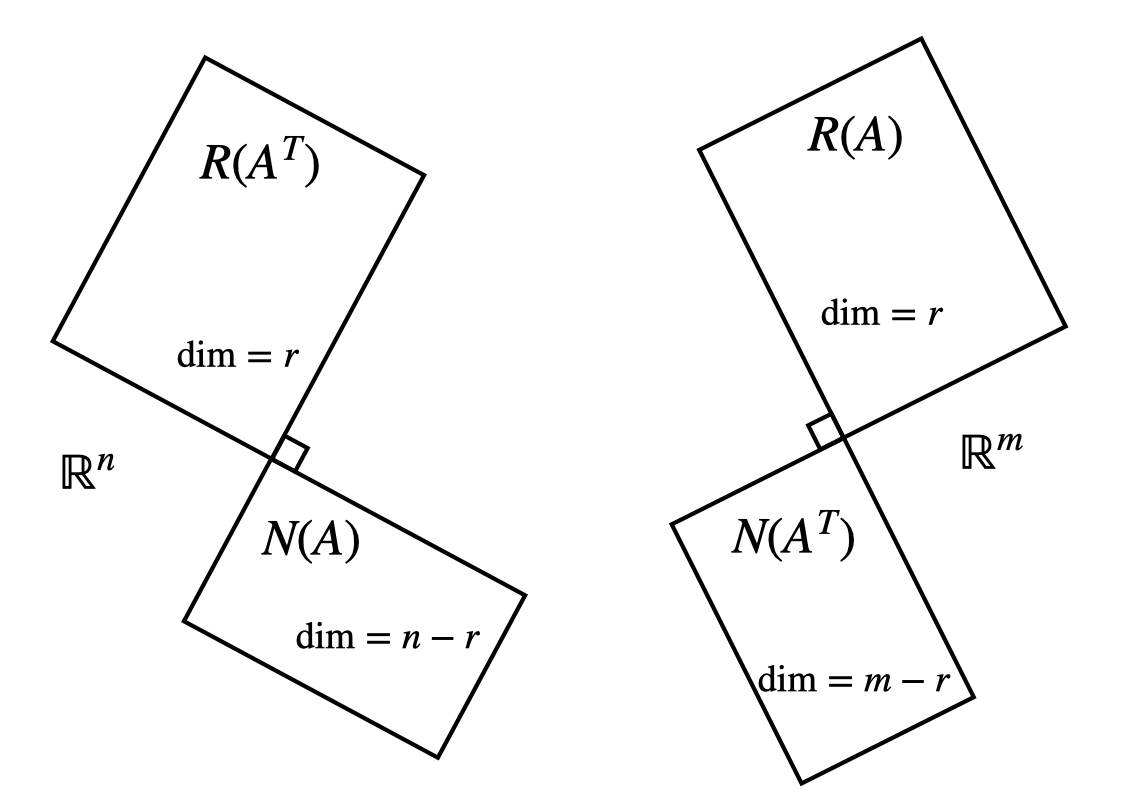
\includegraphics[width=0.55\linewidth]{figs/spaces.png}
\end{figure}
\end{remark}

\begin{definition}[正交变换]
设 $V$ 是一个欧式空间,$T$ 为其上的线性变换。若 $T$ 保持 $V$ 中任意向量 $x$ 长度不变,即 $\Vert Tx\Vert=\Vert x\Vert$,则称 $T$ 为正交变换。
\end{definition}

\begin{theorem}[正交变换的等价定义]
欧式空间 $V$ 上的线性变换 $T$ 是正交变换的充要条件是保持内积不变,即对任意 $x,y\in V$,有 $(Tx,Ty)=(x,y)$.
\end{theorem}

\begin{definition}[正交矩阵]
若方阵 $Q$ 满足:$Q^TQ=I$ 或 $Q^{-1}=Q^T$.  即 $Q$ 各列向量标准正交,则称 $Q$ 为正交矩阵。
\end{definition}

\begin{theorem}[正交变换与正交矩阵]
欧式空间上的线性变换 $T$ 为正交变换的充要条件是其在\textbf{标准正交基}下的矩阵表示是正交矩阵。
\end{theorem}
\begin{proof}
设 $X$ 为一个标准正交基,$TX=XA$,任取 $x=X\alpha$,则 $Tx=TX\alpha=XA\alpha$,因此:
\begin{align*}
    &(Tx,Tx)=(A\alpha)^T(A\alpha)=\alpha^TA^TA\alpha=(x,x)=\alpha^T\alpha\\
    \iff\;&\alpha^T(I-A^TA)\alpha=0\\
    \iff\;& A^TA=I
\end{align*}
\end{proof}
\begin{note}
注意定理成立必须是在标准正交基下。
\end{note}

\begin{property}
正交矩阵非奇异。
\end{property}

\begin{property}
正交矩阵的逆仍为正交矩阵。
\end{property}

\begin{property}
正交矩阵的乘积仍为正交矩阵。
\end{property}

\begin{property}
正交基变换矩阵为正交矩阵。
\end{property}
\begin{proof}
设 $X,Y$ 为正交基,$Y=XC$,任取 $x=Y\alpha=XC\alpha,\,y=Y\beta=XC\beta$,则:
\[
    (x,y)=\alpha^T\beta=(C\alpha)^T(C\beta)=\alpha^T(C^TC)\beta\implies C^TC=I
\]
\end{proof}

\begin{property}
正交矩阵的特征值位于复平面的单位圆上。
\end{property}
\begin{proof}
设 $A$ 为正交矩阵,$Ax=\lambda x\ (x\neq 0)$,则两边取共轭转置得 $x^HA^T=\bar\lambda x^H$(注意 $A$ 是实矩阵,但其特征值和特征向量可能是复数)。于是:
\[
    x^Hx=x^HA^TAx=\lambda\bar\lambda x^Hx=|\lambda|^2x^Hx\implies |\lambda|^2=1
\]
\end{proof}

\begin{definition}[线性映射的共轭]
设 $P$ 是欧氏空间 $W$ 到欧氏空间 $V$ 的一个线性映射,$Q$ 是 $V$ 到 $W$ 的一个线性映射,若对 $\forall x\in W,y\in V$,有 $(Px,y)=(x,Qy)$,则称 $Q$ 为 $P$ 的共轭。
\end{definition}

\begin{figure}[H]
    \centering
    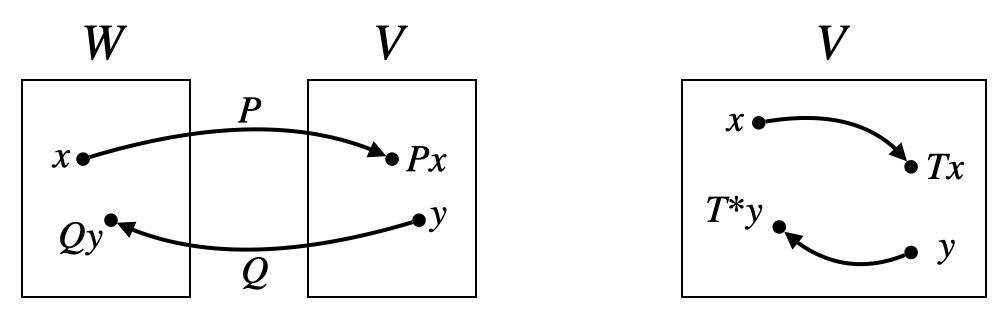
\includegraphics[width=0.5\linewidth]{figs/conj.png}
\end{figure}

\begin{theorem}
设 $X,Y$ 分别是欧式空间 $W,V$ 的标准正交基,$P$ 是 $W$ 到 $V$ 的一个线性映射,$Q$ 是 $P$ 的共轭。设 $P,Q$ 在 $X,Y$ 下的矩阵表示为 $A,B$,则 $B=A^T$.
\end{theorem}
\begin{proof}
由于 $PX=YA,\,QY=XB$,所以:
\begin{gather*}
    (Px_j,y_i)=\left(\sum_{k=1}^m a_{kj}y_k,y_i\right)=a_{ij}\\
    (x_j,Qy_i)=\left(x_j,\sum_{k=1}^nb_{ki}x_k\right)=b_{ji}
\end{gather*}
由于 $(Px_j,y_i)=(x_j,Qy_i)$,故 $a_{ij}=b_{ji}$,即 $B=A^T$.
\end{proof}

\begin{definition}[线性变换的共轭]
设 $T$ 是欧氏空间 $V$ 上的一个线性变换,若对 $\forall x,y\in V$,有 $(Tx,y)=(x,T^\ast y)$ 成立,则称 $T^\ast$ 为 $T$ 的共轭。
\end{definition}

\begin{theorem}
\label{thm:conjgram}
设 $T$ 在基 $X=(x_1,\ldots,x_n)$ 下的矩阵表示为 $A$,$X$ 的 Gram 矩阵为 $C$,那么 $T^\ast$ 在基 $X$ 下的矩阵表示为 $B=C^{-1}A^TC$.
\end{theorem}
\begin{proof}
由于 $TX=XA,\,T^\ast X=XB$,所以:
\begin{gather*}
    (Tx_i,x_j)=\left(\sum_{k=1}^na_{ki}x_k,x_j\right)=\sum_{k=1}^na_{ki}(x_k,x_j)=\sum_{k=1}^na_{ki}c_{kj}\\
    (x_i,T^\ast x_j)=\left(x_i,\sum_{k=1}^nb_{kj}x_k\right)=\sum_{k=1}^nb_{kj}(x_i,x_k)=\sum_{k=1}^nb_{kj}c_{ik}\\
\end{gather*}
得 $\sum_{k=1}^na_{ki}c_{kj}=\sum_{k=1}^n b_{kj}c_{ik}$,即 $A^TC=CB$.
\end{proof}

\begin{definition}[实对称变换]
设 $T$ 是欧氏空间 $V$ 的一个线性变换,且对 $V$ 中任意两个向量 $x,y$ 都有 $(Tx,y)=(x,Ty)$ 成立,则称 $T$ 为 $V$ 中一个实对称变换。
\end{definition}

\begin{theorem}[实对称变换与实对称矩阵]
欧氏空间中的线性变换是实对称变换的充要条件是它在\textbf{标准正交基}下的矩阵为实对称矩阵。
\end{theorem}
\begin{proof}
设 $X$ 为一个标准正交基,设 $T$ 在 $X$ 下的矩阵表示为 $A$,即 $TX=XA$.

必要性:由于 $X$ 为标准正交基,故其 Gram 矩阵为 $I$,由于 $T$ 本身就是自己的共轭,根据定理 \ref{thm:conjgram} 可知 $A=I^{-1}A^TI=A^T$.

充分性:
\begin{gather*}
(Tx_i,x_j)=\left(\sum_{k=1}^na_{ki}x_k,x_j\right)=a_{ji}\\
(x_i,Tx_j)=\left(x_i,\sum_{k=1}^na_{kj}x_k\right)=a_{ij}
\end{gather*}
得 $a_{ji}=a_{ij}$.
\end{proof}

\begin{theorem}
实对称矩阵特征值都为实数,属于不同特征值的特征向量相互正交。
\end{theorem}
\begin{proof}
设 $Ax=\lambda x\ (x\neq 0)$,则:
\[
x^HAx=\lambda x^Hx=(A^Hx)^Hx=(Ax)^Hx=(\lambda x)^Hx=\bar\lambda x^Hx\implies \lambda=\bar\lambda
\]
故 $\lambda\in\mathbb R$.
再设 $Ay=\mu y\ (y\neq 0)$ 且 $\lambda\neq \mu$,则:
\[
y^TAx=\lambda y^Tx=(A^Ty)^Tx=(Ay)^Tx=\mu y^Tx\implies y^Tx=0
\]
\end{proof}

下面我们将线性空间的数域从实数域扩展到复数域,那么相应的,欧式空间扩展为酉空间,内积扩展为复内积,正交变换和正交矩阵扩展为酉变换和酉矩阵,实对称变换和实对称矩阵扩展为 Hermite 矩阵和 Hermite 变换。它们都有着类似的性质。

\begin{definition}[酉空间,复内积]
设 $V$ 是复数域 $C$ 上的线性空间,对 $V$ 中任意 $x$ 和 $y$,按某种规则定义一个复数,用 $(x,y)$ 表示,且满足下列四个条件:
\begin{itemize}
    \item 交换律:$(x,y)=\overline{(y,x)}$
    \item 分配律:$(x,y+z)=(x,y)+(x,z)$
    \item 齐次性:$(kx,y)=k(x,y),\,\forall k\in \mathbb C$
    \item 非负性:$(x,x)\geq 0$,当且仅当 $x=0$ 时 $(x,x)=0$
\end{itemize}
则称 $(x,y)$ 为复内积,$V$ 为酉空间、复欧氏空间或复内积空间。
\end{definition}

\begin{example}[根据坐标定义复内积]
设 $X$ 为 $V$ 上的一个基,向量 $x,y\in V$ 在该基下的坐标分别为 $\alpha=(\alpha_1,\ldots,\alpha_n)^T,\beta=(\beta_1,\ldots,\beta_n)^T$,则可以定义内积为:
\[
    (x,y)=\alpha_1\bar\beta_1+\cdots+\alpha_n\bar\beta_n=\beta^H\alpha
\]
容易验证这确实满足内积的四个条件。
\end{example}
\begin{note}
注意共轭转置取在 $\beta$ 上,这是为了满足齐次性而导致的。在有些教材上,齐次性写作 $(x,ky)=k(x,y)$,则内积相应地会变成 $\alpha^H\beta$,共轭转置取在 $\alpha$ 上。
\end{note}

\begin{definition}[酉变换]
设 $T$ 是酉空间 $V$ 中的线性变换,若 $T$ 保持长度不变,即对 $V$ 中任意 $x$,有 $(Tx,Tx)=(x,x)$,则称 $T$ 为 $V$ 上的酉变换。
\end{definition}

\begin{theorem}[酉变换的等价定义]
酉空间 $V$ 上的线性变换 $T$ 是酉变换的充要条件是保持内积不变,即对任意 $x,y\in V$,有 $(Tx,Ty)=(x,y)$.
\end{theorem}

\begin{definition}[酉矩阵]
若 $n$ 阶矩阵 $A$ 满足 $A^HA=AA^H=I$,则称 $A$ 为酉矩阵。
\end{definition}

\begin{theorem}[酉变换与酉矩阵]
酉变换在酉空间的\textbf{标准正交基}下的矩阵是酉矩阵。
\end{theorem}

\begin{property}
酉矩阵的逆矩阵也是酉矩阵。
\end{property}

\begin{property}
两个酉矩阵的乘积也是酉矩阵。
\end{property}

\begin{definition}[复线性映射的共轭]
设 $P$ 是酉空间 $W$ 到酉空间 $V$ 的一个线性映射,$Q$ 是酉空间
$V$ 到酉空间 $W$ 的一个线性映射,若对 $\forall x\in W,y\in V$,有 $(Px,y)=(x,Qy)$,则称 $Q$ 为 $P$ 的共轭。
\end{definition}

\begin{theorem}
设 $X,Y$ 分别是酉空间 $W,V$ 的标准正交基,$P$ 是 $W$ 到 $V$ 的一个线性映射,$Q$ 是 $P$ 的共轭。设 $P,Q$ 在 $X,Y$ 下的矩阵表示为 $A,B$,则 $B=A^H$.
\end{theorem}

\begin{definition}[复线性变换的共轭]
设 $T$ 是酉空间 $V$ 上的一个线性变换,若对 $\forall x,y\in V$,有 $(Tx,y)=(x,T^\ast y)$ 成立,则称 $T^\ast$ 为 $T$ 的共轭。
\end{definition}

\begin{property}
线性变换 $T$ 的共轭仍是线性变换。
\end{property}
\begin{theorem}
设 $T$ 在基 $X=(x_1,\ldots,x_n)$ 下的矩阵表示为 $A$,$X$ 的 Gram 矩阵为 $C$,那么 $T^\ast$ 在基 $X$ 下的矩阵表示为 $B=C^{-1}A^HC$.
\end{theorem}

\begin{definition}[Hermite 变换/酉对称变换]
设 $T$ 为酉空间 $V$ 上的线性变换,若满足对任意 $x,y\in V$,都有 $(Tx,y)=(x,Ty)$,则称 $T$ 为 Hermite 变换或酉对称变换。
\end{definition}

\begin{definition}[Hermite 矩阵]
若 $n$ 阶矩阵 $A$ 满足 $A=A^H$,则称 $A$ 为 Hermite 矩阵。
\end{definition}

\begin{theorem}[Hermite 变换与 Hermite 矩阵]
Hermite 变换在\textbf{标准正交基}下的矩阵是 Hermite 矩阵。
\end{theorem}

\begin{theorem}
Hermite 矩阵的特征值都是实数,属于不同特征值的特征向量相互正交。
\end{theorem}

\begin{theorem}[Schur 定理]
\label{thm:schur}
\ 

1) 设 $A\in\mathbb C^{n\times n}$,则存在酉矩阵 $P$ 使得 $P^HAP=U$,其中 $U$ 为上三角矩阵。

2) 设 $A\in\mathbb R^{n\times n}$ 且所有特征值为实数,则存在正交矩阵 $Q$ 使得 $Q^TAQ=U$,其中 $U$ 为上三角矩阵。
\end{theorem}

\begin{remark}
在定理 \ref{thm:anysimilar} 中,我们证明了任意矩阵都相似于一个上三角矩阵。Schur 定理是该定理的加强版,它限制用来相似化的矩阵是一个酉矩阵。Schur 定理的证明过程与定理 \ref{thm:anysimilar} 是类似的,只不过基扩充时需要扩充为标准正交基,所有的可逆矩阵换成酉矩阵。
\end{remark}

\begin{definition}[正规矩阵]
设 $A\in\mathbb C^{n\times n}$ 且 $A^HA=AA^H$,称 $A$ 为正规矩阵。
\end{definition}
\begin{remark}
式 $A^HA=AA^H$ 意味着 $A$ 的 $i,j$ 行内积等于 $i,j$ 列内积。因此,前面提到的\textbf{正交矩阵、对称矩阵、酉矩阵、Hermite 矩阵都是正规矩阵}。
\end{remark}

\begin{theorem}[正规矩阵的充要条件]
\label{thm:unisim}
\ 

1) 设 $A\in\mathbb C^{n\times n}$,则 $A$ 为正规矩阵的充要条件为 $A$ 酉相似于对角矩阵,即存在酉矩阵 $P$ 使得 $P^HAP=D$,其中 $D$ 为对角矩阵。

2) 设 $A\in\mathbb R^{n\times n}$ 且所有特征值为实数,则 $A$ 为正规矩阵的充要条件为 $A$ 正交相似于对角矩阵,即存在正交矩阵 $Q$ 使得 $Q^TAQ=D$,其中 $D$ 为对角矩阵。
\end{theorem}
\begin{proof}
只证明 1),2) 类似可证。充分性易证;对于必要性,根据 Schur 定理 \ref{thm:schur},$A$ 酉相似于一个上三角矩阵:$P^HAP=U$. 容易证明,$A$ 正规 $\iff$ $U$ 正规,于是 $U^HU=UU^H$,故 $U$ 只能是对角矩阵。
\end{proof}

\begin{corollary}
实对称矩阵正交相似于对角矩阵。
\end{corollary}

% \begin{theorem}[Hermite 矩阵的谱分解]
% 设 $A$ 为 Hermite 矩阵,$\lambda_i,p_i$ 是 $A$ 的特征值和特征向量,则:
% \[
%     A=\lambda_1p_1p_1^H+\cdots+\lambda_np_np_n^H=P\Lambda P^H
% \]
% \end{theorem}
